\documentclass[11pt,fleqn]{book} % Default font size and left-justified equations

\usepackage[top=3cm,bottom=3cm,left=3.2cm,right=3.2cm,headsep=10pt,letterpaper]{geometry} % Page margins

\usepackage{xcolor} % Required for specifying colors by name
\definecolor{ocre}{RGB}{52,177,201} % Define the orange color used for highlighting throughout the book%

% Font Settings
\usepackage{avant} % Use the Avantgarde font for headings
%\usepackage{times} % Use the Times font for headings
\usepackage{mathptmx} % Use the Adobe Times Roman as the default text font together with math symbols from the Sym­bol, Chancery and Com­puter Modern fonts
\usepackage{microtype} % Slightly tweak font spacing for aesthetics
\usepackage[utf8]{inputenc} % Required for including letters with accents
\usepackage[T1]{fontenc} % Use 8-bit encoding that has 256 glyphs
%%%

%% Bibliography
%\usepackage[style=alphabetic,sorting=nyt,sortcites=true,autopunct=true,babel=hyphen,hyperref=true,abbreviate=false,backref=true,backend=biber]{biblatex}
%\addbibresource{biblio.bib} % BibTeX bibliography file
%\defbibheading{bibempty}{}

%----------------------------------------------------------------------------------------
%	VARIOUS REQUIRED PACKAGES
%----------------------------------------------------------------------------------------

\usepackage{titlesec} % Allows customization of titles

\usepackage{graphicx} % Required for including pictures
\graphicspath{{Pictures/}} % Specifies the directory where pictures are stored
% \graphicspath{{Plots/}}
\usepackage{lipsum} % Inserts dummy text

\usepackage{tikz} % Required for drawing custom shapes

\usepackage[english]{babel} % English language/hyphenation

\usepackage{enumitem} % Customize lists
\setlist{nolistsep} % Reduce spacing between bullet points and numbered lists

\usepackage{booktabs} % Required for nicer horizontal rules in tables

\usepackage{eso-pic} % Required for specifying an image background in the title page

%----------------------------------------------------------------------------------------
%	MAIN TABLE OF CONTENTS
%----------------------------------------------------------------------------------------

\usepackage{titletoc} % Required for manipulating the table of contents

\contentsmargin{0cm} % Removes the default margin
% Chapter text styling
\titlecontents{chapter}[1.25cm] % Indentation
{\addvspace{15pt}\large\sffamily\bfseries} % Spacing and font options for chapters
{\color{ocre!60}\contentslabel[\Large\thecontentslabel]{1.25cm}\color{ocre}} % Chapter number
{}  
{\color{ocre!60}\normalsize\sffamily\bfseries\;\titlerule*[.5pc]{.}\;\thecontentspage} % Page number
% Section text styling
\titlecontents{section}[1.25cm] % Indentation
{\addvspace{5pt}\sffamily\bfseries} % Spacing and font options for sections
{\contentslabel[\thecontentslabel]{1.25cm}} % Section number
{}
{\sffamily\hfill\color{black}\thecontentspage} % Page number
[]
% Subsection text styling
\titlecontents{subsection}[1.25cm] % Indentation
{\addvspace{1pt}\sffamily\small} % Spacing and font options for subsections
{\contentslabel[\thecontentslabel]{1.25cm}} % Subsection number
{}
{\sffamily\;\titlerule*[.5pc]{.}\;\thecontentspage} % Page number
[] 

%----------------------------------------------------------------------------------------
%	MINI TABLE OF CONTENTS IN CHAPTER HEADS
%----------------------------------------------------------------------------------------

% Section text styling
\titlecontents{lsection}[0em] % Indendating
{\footnotesize\sffamily} % Font settings
{}
{}
{}

% Subsection text styling
\titlecontents{lsubsection}[.5em] % Indentation
{\normalfont\footnotesize\sffamily} % Font settings
{}
{}
{}
 
%----------------------------------------------------------------------------------------
%	PAGE HEADERS
%----------------------------------------------------------------------------------------

\usepackage{fancyhdr} % Required for header and footer configuration

\pagestyle{fancy}
\renewcommand{\chaptermark}[1]{\markboth{\sffamily\normalsize\bfseries\chaptername\ \thechapter.\ #1}{}} % Chapter text font settings
\renewcommand{\sectionmark}[1]{\markright{\sffamily\normalsize\thesection\hspace{5pt}#1}{}} % Section text font settings
\fancyhf{} \fancyhead[LE,RO]{\sffamily\normalsize\thepage} % Font setting for the page number in the header
\fancyhead[LO]{\rightmark} % Print the nearest section name on the left side of odd pages
\fancyhead[RE]{\leftmark} % Print the current chapter name on the right side of even pages
\renewcommand{\headrulewidth}{0.5pt} % Width of the rule under the header
\addtolength{\headheight}{2.5pt} % Increase the spacing around the header slightly
\renewcommand{\footrulewidth}{0pt} % Removes the rule in the footer
\fancypagestyle{plain}{\fancyhead{}\renewcommand{\headrulewidth}{0pt}} % Style for when a plain pagestyle is specified

% Removes the header from odd empty pages at the end of chapters
\makeatletter
\renewcommand{\cleardoublepage}{
\clearpage\ifodd\c@page\else
\hbox{}
\vspace*{\fill}
\thispagestyle{empty}
\newpage
\fi}

%----------------------------------------------------------------------------------------
%	THEOREM STYLES
%----------------------------------------------------------------------------------------

\usepackage{amsmath,amsfonts,amssymb,amsthm} % For math equations, theorems, symbols, etc

\newcommand{\intoo}[2]{\mathopen{]}#1\,;#2\mathclose{[}}
\newcommand{\ud}{\mathop{\mathrm{{}d}}\mathopen{}}
\newcommand{\intff}[2]{\mathopen{[}#1\,;#2\mathclose{]}}
\newtheorem{notation}{Notation}[chapter]

%%%%%%%%%%%%%%%%%%%%%%%%%%%%%%%%%%%%%%%%%%%%%%%%%%%%%%%%%%%%%%%%%%%%%%%%%%%
%%%%%%%%%%%%%%%%%%%% dedicated to boxed/framed environements %%%%%%%%%%%%%%
%%%%%%%%%%%%%%%%%%%%%%%%%%%%%%%%%%%%%%%%%%%%%%%%%%%%%%%%%%%%%%%%%%%%%%%%%%%
\newtheoremstyle{ocrenumbox}% % Theorem style name
{0pt}% Space above
{0pt}% Space below
{\normalfont}% % Body font
{}% Indent amount
{\small\bf\sffamily\color{ocre}}% % Theorem head font
{\;}% Punctuation after theorem head
{0.25em}% Space after theorem head
{\small\sffamily\color{ocre}\thmname{#1}\nobreakspace\thmnumber{\@ifnotempty{#1}{}\@upn{#2}}% Theorem text (e.g. Theorem 2.1)
\thmnote{\nobreakspace\the\thm@notefont\sffamily\bfseries\color{black}---\nobreakspace#3.}} % Optional theorem note
\renewcommand{\qedsymbol}{$\blacksquare$}% Optional qed square

\newtheoremstyle{blacknumex}% Theorem style name
{5pt}% Space above
{5pt}% Space below
{\normalfont}% Body font
{} % Indent amount
{\small\bf\sffamily}% Theorem head font
{\;}% Punctuation after theorem head
{0.25em}% Space after theorem head
{\small\sffamily{\tiny\ensuremath{\blacksquare}}\nobreakspace\thmname{#1}\nobreakspace\thmnumber{\@ifnotempty{#1}{}\@upn{#2}}% Theorem text (e.g. Theorem 2.1)
\thmnote{\nobreakspace\the\thm@notefont\sffamily\bfseries---\nobreakspace#3.}}% Optional theorem note

\newtheoremstyle{blacknumbox} % Theorem style name
{0pt}% Space above
{0pt}% Space below
{\normalfont}% Body font
{}% Indent amount
{\small\bf\sffamily}% Theorem head font
{\;}% Punctuation after theorem head
{0.25em}% Space after theorem head
{\small\sffamily\thmname{#1}\nobreakspace\thmnumber{\@ifnotempty{#1}{}\@upn{#2}}% Theorem text (e.g. Theorem 2.1)
\thmnote{\nobreakspace\the\thm@notefont\sffamily\bfseries---\nobreakspace#3.}}% Optional theorem note

%%%%%%%%%%%%%%%%%%%%%%%%%%%%%%%%%%%%%%%%%%%%%%%%%%%%%%%%%%%%%%%%%%%%%%%%%%%
%%%%%%%%%%%%% dedicated to non-boxed/non-framed environements %%%%%%%%%%%%%
%%%%%%%%%%%%%%%%%%%%%%%%%%%%%%%%%%%%%%%%%%%%%%%%%%%%%%%%%%%%%%%%%%%%%%%%%%%
\newtheoremstyle{ocrenum}% % Theorem style name
{5pt}% Space above
{5pt}% Space below
{\normalfont}% % Body font
{}% Indent amount
{\small\bf\sffamily\color{ocre}}% % Theorem head font
{\;}% Punctuation after theorem head
{0.25em}% Space after theorem head
{\small\sffamily\color{ocre}\thmname{#1}\nobreakspace\thmnumber{\@ifnotempty{#1}{}\@upn{#2}}% Theorem text (e.g. Theorem 2.1)
\thmnote{\nobreakspace\the\thm@notefont\sffamily\bfseries\color{black}---\nobreakspace#3.}} % Optional theorem note
\renewcommand{\qedsymbol}{$\blacksquare$}% Optional qed square
\makeatother

% Defines the theorem text style for each type of theorem to one of the three styles above
\newcounter{dummy} 
\numberwithin{dummy}{section}
\theoremstyle{ocrenumbox}


\newtheorem{theoremeT}[dummy]{Theorem}
\newtheorem{lemma}[dummy]{Lemma}
\newtheorem{observation}[dummy]{Observation}
\newtheorem{proposition}[dummy]{Proposition}
% \newtheorem{definition}[dummy]{Definition}
\newtheorem{claim}[dummy]{Claim}
\newtheorem{fact}[dummy]{Fact}
\newtheorem{assumption}[dummy]{Assumption}

\newtheorem{problem}{Problem}[chapter]
% \newtheorem{exercise}{Exercise}[chapter]
\theoremstyle{blacknumex}
\newtheorem{exampleT}{Example}[chapter]
\theoremstyle{blacknumbox}
\newtheorem{vocabulary}{Vocabulary}[chapter]
\newtheorem{definitionT}{Definition}[section]
\newtheorem{corollaryT}[dummy]{Corollary}
\theoremstyle{ocrenum}

%----------------------------------------------------------------------------------------
%	DEFINITION OF COLORED BOXES
%----------------------------------------------------------------------------------------

\RequirePackage[framemethod=default]{mdframed} % Required for creating the theorem, definition, exercise and corollary boxes

% Theorem box
\newmdenv[skipabove=7pt,
skipbelow=7pt,
backgroundcolor=black!5,
linecolor=ocre,
innerleftmargin=5pt,
innerrightmargin=5pt,
innertopmargin=5pt,
leftmargin=0cm,
rightmargin=0cm,
innerbottommargin=5pt]{tBox}

% Exercise box	  
\newmdenv[skipabove=7pt,
skipbelow=7pt,
rightline=false,
leftline=true,
topline=false,
bottomline=false,
backgroundcolor=ocre!10,
linecolor=ocre,
innerleftmargin=5pt,
innerrightmargin=5pt,
innertopmargin=5pt,
innerbottommargin=5pt,
leftmargin=0cm,
rightmargin=0cm,
linewidth=4pt]{eBox}	

% Definition box
\newmdenv[skipabove=7pt,
skipbelow=7pt,
rightline=false,
leftline=true,
topline=false,
bottomline=false,
linecolor=ocre,
innerleftmargin=5pt,
innerrightmargin=5pt,
innertopmargin=0pt,
leftmargin=0cm,
rightmargin=0cm,
linewidth=4pt,
innerbottommargin=0pt]{dBox}	

% Corollary box
\newmdenv[skipabove=7pt,
skipbelow=7pt,
rightline=false,
leftline=true,
topline=false,
bottomline=false,
linecolor=gray,
backgroundcolor=black!5,
innerleftmargin=5pt,
innerrightmargin=5pt,
innertopmargin=5pt,
leftmargin=0cm,
rightmargin=0cm,
linewidth=4pt,
innerbottommargin=5pt]{cBox}

% Creates an environment for each type of theorem and assigns it a theorem text style from the "Theorem Styles" section above and a colored box from above
\newenvironment{theorem}{\begin{tBox}\begin{theoremeT}}{\end{theoremeT}\end{tBox}}
\newenvironment{exercise}{\begin{eBox}\begin{exerciseT}}{\hfill{\color{ocre}\tiny\ensuremath{\blacksquare}}\end{exerciseT}\end{eBox}}				  
\newenvironment{definition}{\begin{dBox}\begin{definitionT}}{\end{definitionT}\end{dBox}}	
\newenvironment{example}{\begin{exampleT}}{\hfill{\tiny\ensuremath{\blacksquare}}\end{exampleT}}		
\newenvironment{corollary}{\begin{cBox}\begin{corollaryT}}{\end{corollaryT}\end{cBox}}
\newtheorem{solution}{Solution}[chapter]
\newtheorem{exerciseT}{Exercise}[chapter]

%----------------------------------------------------------------------------------------
%	REMARK ENVIRONMENT
%----------------------------------------------------------------------------------------

\newenvironment{remark}{\par\vspace{10pt}\small % Vertical white space above the remark and smaller font size
\begin{list}{}{
\leftmargin=35pt % Indentation on the left
\rightmargin=25pt}\item\ignorespaces % Indentation on the right
\makebox[-2.5pt]{\begin{tikzpicture}[overlay]
\node[draw=ocre!60,line width=1pt,circle,fill=ocre!25,font=\sffamily\bfseries,inner sep=2pt,outer sep=0pt] at (-15pt,0pt){\textcolor{ocre}{R}};\end{tikzpicture}} % Orange R in a circle
\advance\baselineskip -1pt}{\end{list}\vskip5pt} % Tighter line spacing and white space after remark

%----------------------------------------------------------------------------------------
%	SECTION NUMBERING IN THE MARGIN
%----------------------------------------------------------------------------------------

\makeatletter
\renewcommand{\@seccntformat}[1]{\llap{\textcolor{ocre}{\csname the#1\endcsname}\hspace{1em}}}                    
\renewcommand{\section}{\@startsection{section}{1}{\z@}
{-4ex \@plus -1ex \@minus -.4ex}
{1ex \@plus.2ex }
{\normalfont\large\sffamily\bfseries}}
\renewcommand{\subsection}{\@startsection {subsection}{2}{\z@}
{-3ex \@plus -0.1ex \@minus -.4ex}
{0.5ex \@plus.2ex }
{\normalfont\sffamily\bfseries}}
\renewcommand{\subsubsection}{\@startsection {subsubsection}{3}{\z@}
{-2ex \@plus -0.1ex \@minus -.2ex}
{.2ex \@plus.2ex }
{\normalfont\small\sffamily\bfseries}}                        
\renewcommand\paragraph{\@startsection{paragraph}{4}{\z@}
{-2ex \@plus-.2ex \@minus .2ex}
{.1ex}
{\normalfont\small\sffamily\bfseries}}

%----------------------------------------------------------------------------------------
%	HYPERLINKS IN THE DOCUMENTS
%----------------------------------------------------------------------------------------

% For an unclear reason, the package should be loaded now and not later
\usepackage{hyperref}
\hypersetup{hidelinks,backref=true,pagebackref=true,hyperindex=true,colorlinks=false,breaklinks=true,urlcolor= ocre,bookmarks=true,bookmarksopen=false,pdftitle={Title},pdfauthor={Author}}

%----------------------------------------------------------------------------------------
%	CHAPTER HEADINGS
%----------------------------------------------------------------------------------------

% The set-up below should be (sadly) manually adapted to the overall margin page septup controlled by the geometry package loaded in the main.tex document. It is possible to implement below the dimensions used in the goemetry package (top,bottom,left,right)... TO BE DONE

\newcommand{\thechapterimage}{}
\newcommand{\chapterimage}[1]{\renewcommand{\thechapterimage}{#1}}

% Numbered chapters with mini tableofcontents
\def\thechapter{\arabic{chapter}}
\def\@makechapterhead#1{
\thispagestyle{empty}
{\centering \normalfont\sffamily
\ifnum \c@secnumdepth >\m@ne
\if@mainmatter
\startcontents
\begin{tikzpicture}[remember picture,overlay]
\node at (current page.north west)
{\begin{tikzpicture}[remember picture,overlay]
\node[anchor=north west,inner sep=0pt] at (0,0) {\includegraphics[width=\paperwidth]{\thechapterimage}};
%%%%%%%%%%%%%%%%%%%%%%%%%%%%%%%%%%%%%%%%%%%%%%%%%%%%%%%%%%%%%%%%%%%%%%%%%%%%%%%%%%%%%
% Commenting the 3 lines below removes the small contents box in the chapter heading
%\fill[color=ocre!10!white,opacity=.6] (1cm,0) rectangle (8cm,-7cm);
%\node[anchor=north west] at (1.1cm,.35cm) {\parbox[t][8cm][t]{6.5cm}{\huge\bfseries\flushleft \printcontents{l}{1}{\setcounter{tocdepth}{2}}}};
\draw[anchor=west] (5cm,-9cm) node [rounded corners=20pt,fill=ocre!10!white,text opacity=1,draw=ocre,draw opacity=1,line width=1.5pt,fill opacity=.6,inner sep=12pt]{\huge\sffamily\bfseries\textcolor{black}{\thechapter. #1\strut\makebox[22cm]{}}};
%%%%%%%%%%%%%%%%%%%%%%%%%%%%%%%%%%%%%%%%%%%%%%%%%%%%%%%%%%%%%%%%%%%%%%%%%%%%%%%%%%%%%
\end{tikzpicture}};
\end{tikzpicture}}
\par\vspace*{230\p@}
\fi
\fi}

% Unnumbered chapters without mini tableofcontents (could be added though) 
\def\@makeschapterhead#1{
\thispagestyle{empty}
{\centering \normalfont\sffamily
\ifnum \c@secnumdepth >\m@ne
\if@mainmatter
\begin{tikzpicture}[remember picture,overlay]
\node at (current page.north west)
{\begin{tikzpicture}[remember picture,overlay]
\node[anchor=north west,inner sep=0pt] at (0,0) {\includegraphics[width=\paperwidth]{\thechapterimage}};
\draw[anchor=west] (5cm,-9cm) node [rounded corners=20pt,fill=ocre!10!white,fill opacity=.6,inner sep=12pt,text opacity=1,draw=ocre,draw opacity=1,line width=1.5pt]{\huge\sffamily\bfseries\textcolor{black}{#1\strut\makebox[22cm]{}}};
\end{tikzpicture}};
\end{tikzpicture}}
\par\vspace*{230\p@}
\fi
\fi
}
\makeatother

%----------------------------------------------------------------------------------------
%	LANGUAGE STYLE
%----------------------------------------------------------------------------------------

\usepackage{xcolor} % Required for specifying colors by name
\definecolor{ocre}{RGB}{243,102,25}
\definecolor{deepblue}{rgb}{0,0,0.5}
\definecolor{deepred}{rgb}{0.6,0,0}
\definecolor{deepgreen}{rgb}{0,0.5,0}

% Default fixed font does not support bold face
\DeclareFixedFont{\ttb}{T1}{txtt}{bx}{n}{12} % for bold
\DeclareFixedFont{\ttm}{T1}{txtt}{m}{n}{12}  % for normal
% Python environment
\usepackage{listings}
% Python style for highlighting
\newcommand\pythonstyle{\lstset{
language=Python,
basicstyle=\ttm,
otherkeywords={self},             % Add keywords here
keywordstyle=\ttb\color{deepblue},
emph={MyClass,__init__},          % Custom highlighting
emphstyle=\ttb\color{deepred},    % Custom highlighting style
stringstyle=\color{deepgreen},
frame=tb,                         % Any extra options here
showstringspaces=false            % 
}}

% Python environment
\lstnewenvironment{python}[1][]
{
\pythonstyle
\lstset{#1}
}
{}

% Python for external files
\newcommand\pythonexternal[2][]{{
\pythonstyle
\lstinputlisting[#1]{#2}}}

% Python for inline
\newcommand\pythoninline[1]{{\pythonstyle\lstinline!#1!}}
%%

 % Insert the commands.tex file which contains the majority of the structure behind the template

%----------------------------------------------------------------------------------------
%	Definitions of new commands
%----------------------------------------------------------------------------------------

\begin{document}

%----------------------------------------------------------------------------------------
%	TITLE PAGE
%----------------------------------------------------------------------------------------

\begingroup
\thispagestyle{empty}
\AddToShipoutPicture*{\put(0,0){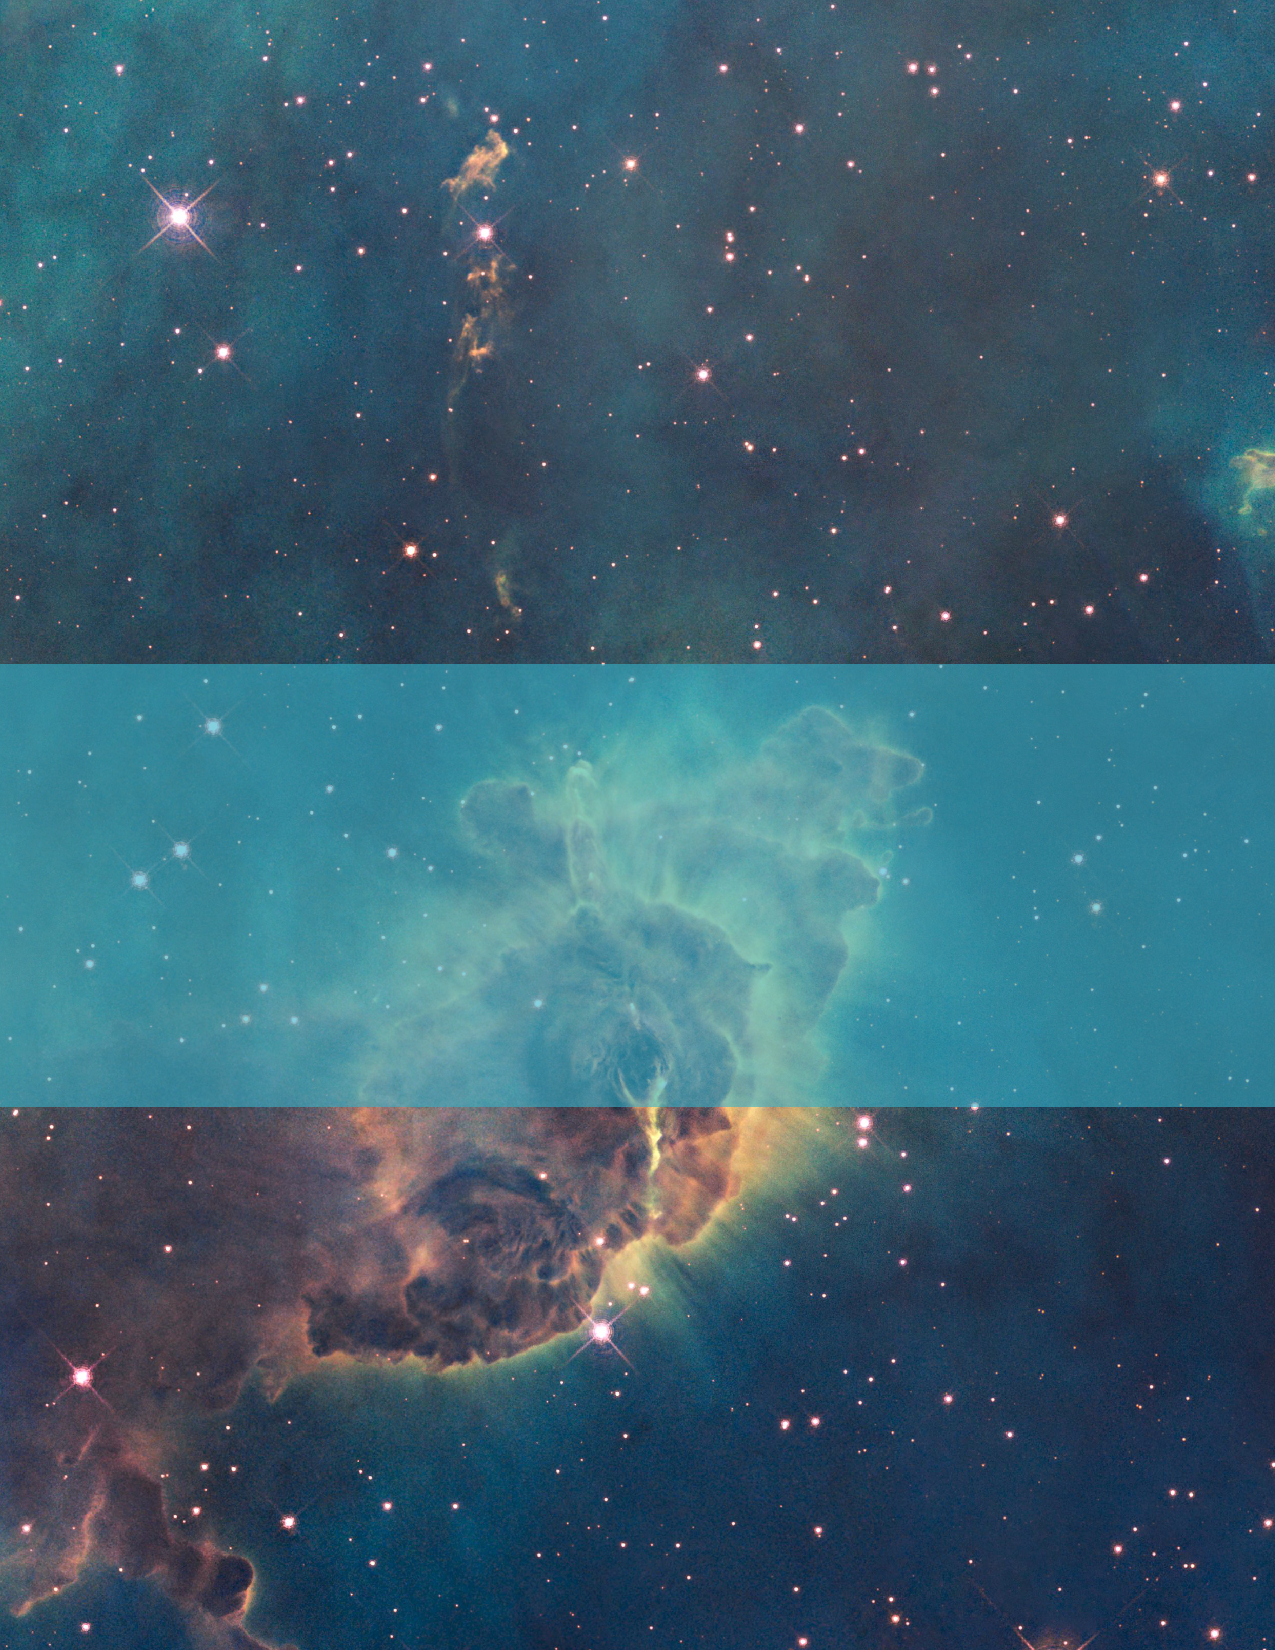
\includegraphics[scale=1.25]{esahubble}}} % Image background
\centering
\vspace*{5cm}
\par\normalfont\fontsize{35}{35}\sffamily\selectfont
\textbf{Le pharaon dans le Coran}\\
{\LARGE Le systeme}\par % Book title
\vspace*{1cm}
{\Huge K.I.A Derouiche}\par % Author name
\endgroup

%----------------------------------------------------------------------------------------
%	COPYRIGHT PAGE
%----------------------------------------------------------------------------------------

\newpage
~\vfill
\thispagestyle{empty}

%----------------------------------------------------------------------------------------
%	TABLE OF CONTENTS
%----------------------------------------------------------------------------------------

\chapterimage{head1.png} % Table of contents heading image

\pagestyle{empty} % No headers

\tableofcontents % Print the table of contents itself

%\cleardoublepage % Forces the first chapter to start on an odd page so it's on the right

\pagestyle{fancy} % Print headers again

%----------------------------------------------------------------------------------------
%	AVANT PROPOS
%----------------------------------------------------------------------------------------

\section{Avant-Propos}
Ce livre traite de SymPy, une bibliothèque de calcul symbolique entièrement écrite en Python un langage 
de programmation de haut niveau, orienté objet, totalement libre, conçu pour produire 
du code de qualité, portable et facile à intégrer. Ainsi la conception d'un programme scientifique  ou 
symbolique avec SymPy et Python est très rapide et offre au développeur une bonne productivité. En tant 
que bibliothèque pythonienne elle repose sur un langage dynamique, très souple d'utilisation et 
constitue un complément idéal à des langages compilés. Elle reste une bibliothèque complète et autosuffisant, pour des petits scripts fonctionnels de quelques lignes, comme pour des applicatifs complexes de plusieurs centaines de modules.

\subsection*{Pourquoi ce livre ?}
Il n'existe pas beaucoup d'ouvrages qui traitent du calcul symbolique en générale par  
rapport aux calculs numériques ou des ouvrages consacré aux bibliothèques symbolique écrite en Python 
est en particulier gravitent autour de SymPy mis à part un livre de 50 pages, quelques chapitres ou des 
lignes de codes cité à titre d'exemples. Citons le livre de référence de Svein Linge et Hans Petter 
Langtangen Programming for Computations – Python A Gentle Introduction to Numerical Simulations with 
Python, aux éditions Springer, ou encore une version du livre de 50 pages Instant SymPy Starter de Ronan 
Lamy, aux éditions Packt Publishing Limited, Le livre est Instant SymPy Starter de Ronan Lamy, c'est un 
guide de démarrage rapide, La documentation en ligne de SymPy est bonne, mais il serait plus facile de 
commencer avec ce livre. Alors, pourquoi ce livre ?

Si ce livre présente comme celui de Ronan Lamy les notions de la bibliothèque, celui-la ajoute des  
exemples originaux, des choix dans la présentation des classes, et une approche globale particulière et 
détaillé, il tente également d’ajouter à ce socle des éléments qui participent de la philosophie de la 
programmation en Python scientifique, aller plus loin dans le développement non scientifique, mettre en 
valeur L’Intérêt et l'importance, à savoir :
\begin{itemize}
 \item des conventions de codage ;
 \item combiné l'approche symbolique et numérique;
 \item des bonnes pratiques de programmation et des techniques d’optimisation ;
\end{itemize}

Même si chacun de ces sujets pourrait à lui seul donner matière à des ouvrages entiers, les réunir dans 
un seul et même livre contribue à fournir une vue complète de ce qu’un développeur d'application 
scientifique en particulier et Python averti et son chef de projet mettent en œuvre quotidiennement.

\subsection*{A qui s'adresse l'ouvrage?}
Cet ouvrage s’adresse bien sûr aux développeurs de tous horizons mais également aux
étudiants,chercheurs, enseignants et chefs de projets. Ils ne trouveront pas dans ce livre de bases de 
programmation; une pratique minimale préalable est indispensable de Python, quel que soit le langage 
utilisé. Il n’est pour autant pas nécessaire de maîtriser la programmation orientée objet et 
la connaissance d’un langage impératif est suffisante.
Les développeurs Python débutants – ou les développeurs avertis ne connaissant pas
encore cette bibliothèque – trouveront dans cet ouvrage des techniques et sujets avancées, les patterns 
efficaces et l’application de certains design patterns objet, topologie, théorie des catégories, machine
learning.
Les étudiants et enseignants trouveront un ouvrage ouvert sur l'apprentissage par l'exercice résolus et 
une interprétation d’exercices mathématiques  
les chercheurs trouveront un outil léger et efficace à travers des approches poussées liées aux 
questions récentes en connections avec les mathématiques pures et appliquées de physique théorique.
Les chefs de projets trouveront des éléments pratiques pour augmenter l’efficacité de
leurs équipes pluridisciplinaires, notamment la présentation des principaux modules à la fois issues de  la bibliothèque standard, graphique et numérique.

\chapterimage{head2.png} % Chapter heading image
\section{Premier pas vers SymPy}
Ce recueil d'exercices et de problèmes de programmation s'adresse aussi bien aux débutants qu'aux programmeurs confirmés. Il présente en effet plusieurs états d'esprit dont les deux principaux sont la programmation classique en Pascal pour les étudiants du premier cycle universitaire, et la programmation fonctionnelle en Lisp pour le second cycle.

Ce livre constitue un panorama (non exhaustif, mais suffisant) sur les langages de programmation, et offre une grande variété dans les sujets traités : graphiques, calcul matriciel, traitements de chaînes de caractères, graphes, intelligence artificielle...
\\
La première partie du livre sera consacré \`a la résolution par une approche symbolique au divers questions posées au étudiants et toute personnes qui aiment savoir et voir s'initier  pour des niveaux et des questions rencontrés, la deuxième partie du livre sera questions aux problèmes plus rencontrés pour des étudiants passionnée des questions entre mathématiques et technologies, chercheurs et développeurs d'applications scientifiques, la troisième partie plus consacré aux questions poussées

\subsection{Pourquoi programmer en symbolique }
Le symbolique est une grande importance d'un point de vue technique, car il permet
de limité les risques de bug dans l'exécution des programmes, dans le contexte de 
la vérification formelle si en prend le programme suivant:

\subsection{Calcul formel}

L'approche La simulation numérique est devenue essentielle dans de nombreux domaines tels que la mécanique des fluides et des solides, la météo, l'évolution du climat, la biologie ou les semi-conducteurs. Elle permet de comprendre, de prévoir, d'accéder là où les instruments de mesures s'arrêtent. 

Ce livre présente des méthodes performantes du calcul scientifique : matrices creuses, résolution efficace des grands systèmes linéaires, ainsi que de nombreuses applications à la résolution par éléments finis et différences finies. Alternant algorithmes et applications, les programmes sont directement présentés en langage C++. Ils sont sous forme concise et claire, et utilisent largement les notions de classe et de généricité du langage C++. 

Le contenu de ce livre a fait l'objet de cours de troisième année à l'école nationale supérieure d'informatique et de mathématiques appliquées de Grenoble (ENSIMAG) ainsi qu'au mystère de mathématiques appliquées de l'université Joseph Fourier. Des connaissances de base d'algèbre matricielle et de programmation sont recommandées. La maîtrise du contenu de cet ouvrage permet d'appréhender les principaux paradigmes de programmation du calcul scientifique. Il est alors possible d'appliquer ces paradigmes pour aborder des problèmes d'intérêt pratique, tels que la résolution des équations aux dérivées partielles, qui est abordée au cours de ce livre. La diversité des sujets abordés, l'efficacité des algorithmes présentés et leur écriture directe en langage C++ font de cet ouvrage un recueil fort utile dans la vie professionnelle d'un ingénieur. 

Le premier chapitre présente les bases fondamentales pour la suite : présentation du langage C++ à travers la conception d'une classe de quaternions et outils d'analyse asymptotique du temps de calcul des algorithmes. Le second chapitre aborde l'algorithme de transformée de Fourier rapide et développe deux applications à la discrétisation d'équations aux dérivées partielles par la méthode des différences finies. Le troisième chapitre est dédié aux matrices creuses et à l'algorithme du gradient conjugué. Ces notions sont appliquées à la méthode des éléments finis. En annexe sont groupés des exemples de génération de maillage et de visualisation graphique. 

S'il est cependant recommandé de maîtriser les notions du premier chapitre pour aborder le reste du livre, les chapitres deux et trois sont complètement indépendants et peuvent être abordés séparément. Ces chapitres sont complétés par des exercices qui en constituent des développements, ainsi que des notes bibliographiques retraçant l'historique des travaux et fournissant des références sur des logiciels et librairies récents implémentant ou étendant les algorithmes présentés. 

\subsection{Un peu de théorie}(source: Wikipédia)
Le calcul formel, ou parfois calcul symbolique, est le domaine des mathématiques et de informatique qui s'intéresse aux algorithmes opérant sur des objets de nature mathématique par le biais de représentations finies et exactes. Ainsi, un nombre entier est représenté de manière finie et exacte par la suite des chiffres de son écriture en base 2. Étant données les représentations de deux nombres entiers, le calcul formel se pose par exemple la question de calculer celle de leur produit.

Le calcul formel est en général considéré comme un domaine distinct du calcul scientifique, cette dernière appellation faisant référence au calcul numérique approché à l'aide de nombres en virgule flottante, là où le calcul formel met l'accent sur les calculs exacts sur des expressions pouvant contenir des variables ou des nombres en précision arbitraire (en). Comme exemples d'opérations de calcul formel, on peut citer le calcul de dérivées ou de primitives, la simplification d'expressions, la décomposition en facteurs irréductibles de polynômes, la mise sous formes normales de matrices, ou encore la résolution des systèmes polynomiaux.

Sur le plan théorique, on s'attache en calcul formel à donner des algorithmes avec la démonstration qu'ils terminent en temps fini et la démonstration que le résultat est bien la représentation d'un objet mathématique défini préalablement. Autant que possible, on essaie de plus d'estimer la complexité des algorithmes que l'on décrit, c'est-à-dire le nombre total d'opérations élémentaires qu'ils effectuent. Cela permet d'avoir une idée a priori du temps d'exécution d'un algorithme, de comparer l'efficacité théorique de différents algorithmes ou encore éclairer la nature même du problème.
\subsection{Logiciel de système de calcul formel}
Dans cette section en va exposer les systèmes de calcul formel, leur intérêt qui à vue un renouveau ces dernières années à cause de l'émergence de technique, technologie et nouvelle approche de programmation pour le domaine scientifique et industriel, hormis le fait que le logiciel de calcul formel en soient sont un outil pédagogique 
indispensable pour les scientifiques et les ingénieurs

\begin{definition}
Un logiciel de système formel est un outil qui facilite le calcul symbolique. La partie principale de ce système est la manipulation des expressions mathématiques sous leur forme symbolique.
\end{definition}

\begin{example}
soit $G=\{x\in\mathbb{R}^2:|x|<3\}$ et noté par: $x^0=(1,1)$; en considère la fonction:
\begin{equation}
f(x)=\left\{\begin{aligned} & \mathrm{e}^{|x|} & & \text{si $|x-x^0|\leq 1/2$}\\
& 0 & & \text{si $|x-x^0|> 1/2$}\end{aligned}\right.
\end{equation}
The function $f$ has bounded support, we can take $A=\{x\in\mathbb{R}^2:|x-x^0|\leq 1/2+\epsilon\}$ for all $\epsilon\in\intoo{0}{5/2-\sqrt{2}}$.
\end{example}

cet exemple se traduit en forme symbolique avec la bibliothèque SymPy:

\subsection{Quelques logiciels de calcul formel}

qui exprime ce qui nous permet notre choix pour un CAS qui possède des caractéristiques techniques et sur le plan du coût très important quand peut résumer dans les points suivants:
\begin{enumerate}
	\item Leger et 
	\item S’appuie sur le langage de programmation Python
	\item Portabilité dans toute transparence
\end{enumerate}

L'un des systèmes qui peut nous permettre d'écrire cette exemple avec un ordinateurs avec SymPy qui semble mieu intégré

\subsection{Bibliothèque SymPy}

Dans un cas plus simple l'exemple 1.1 se formule beaucoup plus dans un outil comme SymPy est une bibliothèque de calcul formel elle est aussi un environnement pour 
l’apprentissage de l’algèbre, l’analyse, géométrie, combinatoire, cryptographie, mécanique 
classique et quantique pour le lycée et l’université mais aussi un environnement de 
développement et de recherche. SymPy  écrit entièrement en Python un langage de 
programmation facile à apprendre et adapté à l’apprentissage,  elle fourni aux étudiant 
\textit{SymPyGamma} une application web   notamment des primitives générales de traitement des expressions algébriques (développement, factorisation, …), des aides à l’organisation des objets mathématiques intervenant dans la résolution d’un problème ainsi qu’une assistance à la preuve. Il permet au professeur de préparer et de suivre le travail de l’élève. Différentes maquettes ont été développées et testées auprès d’élèves. Dans la plus récente, nous nous sommes attachés à explorer une nouvelle forme d’activité algébrique. Alors que le calcul en papier crayon et les logiciels standards considèrent
 les expressions de façon isolée, l’environnement que nous développons organise en réseau les différentes expressions intervenant dans la résolution d’un problème. L’ordinateur peut facilement mettre à jour ce réseau quand l’utilisateur modifie certains de ses éléments. Il devient ainsi possible, pour aborder un problème générique, d’explorer facilement des cas particuliers et de conduire une généralisation. Les relations entre expressions algébriques sont mieux mises en évidence du fait de leur invariance dans les modifications du réseau. De façon très concise, Casyopée peut être défini
\subsubsection{SymPyGamma}
Est une interface onWeb marche avec un navigateur contient plusieurs catégorie liée de calcul, dynamique. L’Intérêt de cette outil qu'il est facilement partageable adapté pour l’enseignement et surtout l'auto-apprentissage 
\subsubsection{Besoin de rester dans le symbolique}
Le symbolique est une grande importance d'un point de vue technique, car il permet
de limité les risques de bug dans l'exécution des programmes, dans le contexte de 
la vérification formelle si en prend le programme suivant:

\subsubsection{Passage du symbolique au numérique}
Généralement, le symbolique parmi c'est  
\subsection{Faire des dessins}



%----------------------------------------------------------------------------------------
%	CHAPTER 1
%----------------------------------------------------------------------------------------
\part{Premier pas vers SymPy}
\chapter{Premier pas vers SymPy}

Ce chapitre d’introduction présente la tournure d'esprit de la bibliothèque mathématique SymPy. Les 
autres chapitres de cette partie développent les notions de base de SymPy: effectuer des calculs 
numériques ou symboliques en analyse, opérer sur des vecteurs et des matrices, écrire des programmes, 
manipuler des listes de données, construire des graphiques, etc. Les parties suivantes de cet ouvrage 
approfondissent quelques branches des mathématiques dans lesquelles l'informatique fait preuve d'ne 
grande efficacité.

\section{La bibliothèque SymPy}

\subsection{Le cas de la bibliothèque SymPy}

Dans un cas plus simple l'exemple 1.1 se formule beaucoup plus dans un outil comme SymPy est une bibliothèque de calcul formel elle est aussi un environnement pour 
l’apprentissage de l'algèbre, l’analyse, géométrie, combinatoire, cryptographie, mécanique 
classique et quantique pour le lycée et l’université mais aussi un environnement de 
développement et de recherche. SymPy  écrit entièrement en Python un langage de 
programmation facile à apprendre et adapté à l’apprentissage,  elle fourni aux étudiant 
\textit{SymPyGamma} une application web   notamment des primitives générales de traitement des 
expressions algébriques (développement, factorisation, …), des aides à l’organisation des objets 
mathématiques intervenant dans la résolution d’un problème ainsi qu’une assistance à la preuve. Il 
permet au professeur de préparer et de suivre le travail de l’élève. Différentes maquettes ont été 
développées et testées auprès d’élèves. Dans la plus récente, nous nous sommes attachés à explorer une 
nouvelle forme d’activité algébrique. Alors que le calcul en papier crayon et les logiciels standards 
considèrent  les expressions de façon isolée, l’environnement que nous développons organise en réseau 
les différentes expressions intervenant dans la résolution d’un problème. L’ordinateur peut facilement 
mettre à jour ce réseau quand l’utilisateur modifie certains de ses éléments. Il devient ainsi possible, 
pour aborder un problème générique, d’explorer facilement des cas particuliers et de conduire une 
généralisation. Les relations entre expressions algébriques sont mieux mises en évidence du fait de leur 
invariance dans les modifications du réseau. De façon très concise, Casyopée peut être défini
\subsection{Travaillez avec SymPy}
\subsection{Installation de SymPy}

\subsection{isympy}
  \begin{python}
IPython console for SymPy 1.3 (Python 3.6.7-64-bit) (ground types: python)
These commands were executed:
>>> from __future__ import division
>>> from sympy import *
>>> x, y, z, t = symbols('x y z t')
>>> k, m, n = symbols('k m n', integer=True)
>>> f, g, h = symbols('f g h', cls=Function)
>>> init_printing()

Documentation can be found at http://docs.sympy.org/1.3/

  \end{python}
\subsection{SymPyGamma}
Est une interface onWeb marche avec un navigateur contient plusieurs catégorie liée de calcul, dynamique. L’Intérêt de cette outil qu'il est facilement partageable adapté pour l’enseignement et surtout l'auto-apprentissage

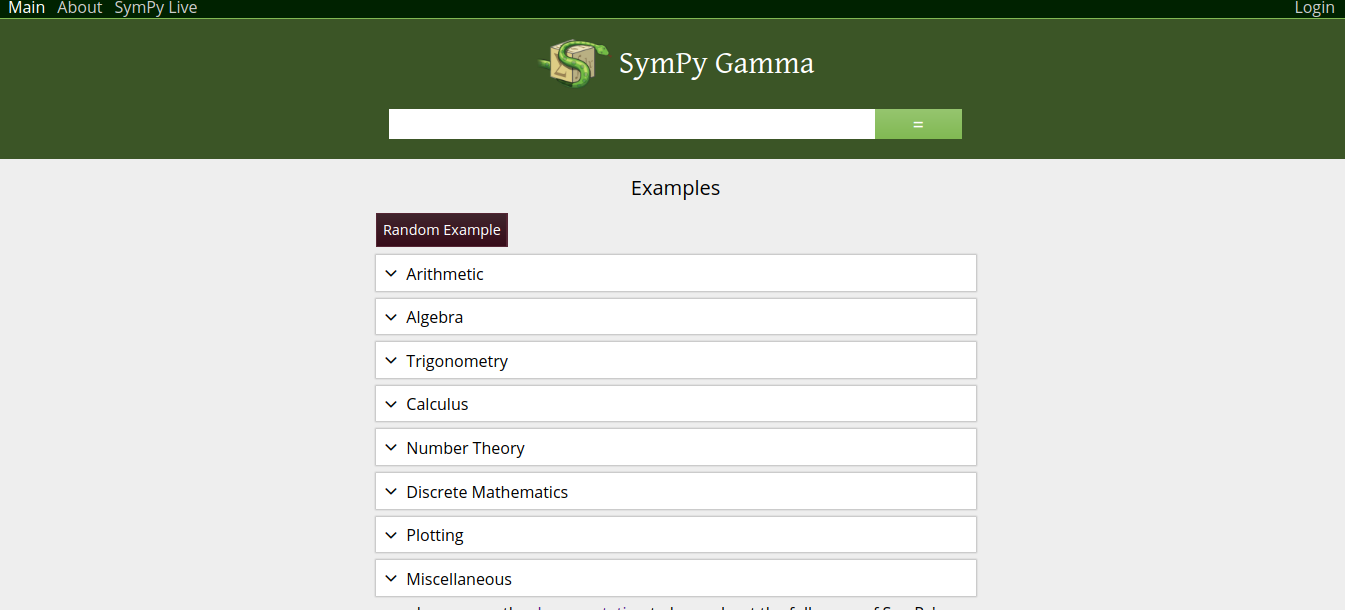
\includegraphics[scale=0.3]{../Pictures/sympyGammaMain.png} 

\subsection{SymPyLive}
SymPy Live est SymPy qui s'exécute sur Google App Engine. Ceci est juste un shell Python standard, avec les commandes suivantes exécutées par défaut
\section{SymPy comme calculatrice}
Contrairement à Sage[], Maple, Octave et les autres logiciel de calcul formel, SymPy, effectue des calculs directe numériques de deux manière différents en passant par la méthode, 
\subsection{Premier calculs}
Dans la suite du livre, nous présentons les calculs sous la forme suivante, qui
imite l’allure d’une session de SymPyLive à travers la ligne de commande isympy:
\begin{python}
In [1]: from sympy import *
In [2]: 1+1                                                                     
Out[2]: 2
\end{python}
\subsubsection{Variables Python}
Lorsque l’on veut conserver le résultat d’un calcul, on peut l’affecter à une
variable :

\subsubsection{Variables Symboliques}
Les objets mathématiques manipulés par SymPy sont symboliques ils sont représentés exactement loin de 
toute approximation numérique, SymPy permet une manipulation avec des expressions contenant
des variables, comme $x^{2} + zy^{3} + z^{2}$ ou encore $sin(x) - exp(x)$. Les variables symboliques
du mathématicien $x$, $y$, $z$ apparaissant dans ces expressions diffèrent, avec SymPy,
des variables du développeur $sin(2) = 0.9092974268256817$ que nous manipulons sous Python 
section précédente. SymPy diffère notablement, sur ce point, d’autres systèmes de calcul
formel comme Maple ou Maxima, Sage c'est inspiré de SymPy sur ce point.
\\

La documentation officiel présente la différence entre valeur numérique gérer par la bibliothèque
standard Python math à travers l'exemple de la racine carré $\sqrt{8}$ sans évaluation,
posons $x=8$

\begin{python}
In [1]: import math                                                             
In [2]: math.sqrt(x)                                                            
Out[2]: 2.8284271247461903
\end{python}
Les variables symboliques doivent \^etre explicitement déclarées avant d'\^etre employées

Dans cet exemple, la commande SR.var(’z’) « construit » et renvoie une variable symbolique dont le nom est z. Cette variable symbolique est un objet Sage comme un autre : elle n’est pas traitée différemment d’expressions plus complexes comme $sin(x) + 1$. Ensuite, cette variable symbolique est affectée à la variable « du programmeur » z, ce qui permet de s’en servir comme de n’importe quelle expression pour construire des expressions plus complexes.


\begin{python}
In [1]: from sympy import *
In [2]: x = symbols('x')                                                                     
In [3]: type(x)
Out[3]: sympy.core.symbol.Symbol
\end{python}

\begin{python}
In [4]: x+3                                                                     
Out[4]: x + 3
\end{python}

\subsection{Structure de données dans SymPy}
Le moteur symbolique de SymPy tire parti de l'orientation des objets (notamment l'héritage) pour créer une base de code facilement extensible. Toutes les classes dérivent des fonctionnalités, telles que la possibilité de se comparer à d'autres objets, à partir de méthodes de la super-classe Basic. Les objets pouvant faire l'objet d'opérations algébriques acquièrent cette capacité grâce à un ensemble de méthodes d'une classe appelée Expr. Ces objets Expr peuvent être conservés dans des objets conteneur (qui contiennent également la sous-classe Expr) Mul, Add et Pow; les objets conteneur sont instanciés à l'aide de l'opérateur Python, tel que la fonction de surcharge, qui permet au constructeur de la classe conteneur d'être appelé chaque fois que l'opérateur binaire approprié est utilisé (* pour Mul, + pour Ajouter et $**$ pour Pow).
De cette manière, des objets supplémentaires peuvent être ajoutés en créant simplement une sous-classe qui hérite des fonctionnalités de la classe Expr. Ces sous-classes bénéficient gratuitement de certaines fonctionnalités, telles que la possibilité de comparer, de multiplier, d’ajouter, etc. Voici comment SymPy crée un environnement modifiable, maintenable, et donc facile à étendre. Grâce à la possibilité d'hériter des propriétés de classes supérieures, la quantité de code nécessaire pour développer, par exemple, un système modélisant la mécanique quantique et la notation Dirac décroissant de manière significative.

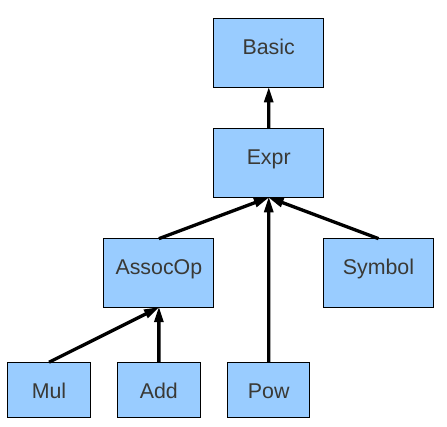
\includegraphics[scale=0.5]{../Pictures/sympyarch.png} 
\subsection{Variable et affection}\index{Variable et affection}

\begin{exercise}
Affectez les variables temps $t$ et distance $d$ par les valeurs 6.892 et 19.7. Calculez et affichez la valeur de la vitesse. Améliorez l'affichage en imposant un chiffre après le point décimal.
\end{exercise}

\begin{solution}
Pour, affectez des variables est les rendre symbolique comme c'est décrit dans le mémo ou il 
sera expliquer temps $t$ et distance $d$ par les valeurs 6.892 et 19.7. Calculez et affichez la 
valeur de la vitesse. Améliorez l'affichage en imposant un chiffre après le point décimal.
\end{solution}

\subsection{Substitution}
Une des choses les plus courantes que vous pourriez vouloir faire avec une expression mathématique est la substitution. La substitution remplace toutes les occurrences de quelque chose dans une expression par quelque chose d'autre. SymPy utilisant la méthode \textbf{subs}. Sym

\subsection{Contrôle du flux d’instructions}\index{Theorems!Single Line}
This is a theorem consisting of just one line.

\begin{exercise}
A set $\mathcal{D}(G)$ in dense in $L^2(G)$, $|\cdot|_0$. 
\end{exercise}
\begin{solution}
\end{solution}
%------------------------------------------------

\chapter{Analyse et Algèbre}\index{Analyse et Algèbre}
Ce chapitre présente à travers des exemples simples les fonctions de base utiles en analyse et en algèbre. Les 
lycéens et étudiants trouveront matière à  remplacer le crayon et le papier par le clavier et l'écran tout en 
relevant le même défi intellectuel de compréhension des mathématiques.Cet exposé des principales commandes de calcul 
avec Sage se veut accessible aux élèves de lycée.

\section{Expressions symboliques et simplification}\index{Expressions symboliques et simplification}
 \subsection{Expressions symboliques}
La bibliothèque SymPy permet d'effectuer toutes sortes de calculs d'analyse à partir d'expressions
symboliques combinant des nombres, des variables symboliques, les quatre opérations, et des fonctions usuelles comme 
sqrt, exp, log, sin, cos, etc. Une expression symbolique peut être représentée par un arbre comme ceux de la. Il est 
important de comprendre qu'une expression symbolique est une formule et non pas une valeur ou une fonction 
mathématique. Ainsi, SymPy ne reconnaît pas que les deux expressions suivantes sont égales
\subsection{Transformation d'expressions}\index{Transformation d'expressions}
\subsection{Fonctions mathématiques usuelles}\index{Fonctions mathématiques usuelles}
La plupart des fonctions mathématiques se retrouvent dans SymPy, en particulier les
fonctions trigonométriques, le logarithme et l'exponentiel : elles sont rassemblées
dans le tableau

\section{Équations}
Ceci est la documentation officielle du module solveset dans les solveurs. Il contient les questions fréquemment posées sur notre nouveau module pour résoudre des équations.
 \subsection{Résolution explicite}\index{Résolution explicite}
 \subsection{Équations sans solution explicite}\index{Équations sans solution explicite}
\section{In\'equations}\index{In\'equations}
\section{Analyse}\index{Analyse}
Dans cette section, nous présentons succinctement les fonctions couramment utiles en analyse réelle. Pour une 
utilisation avancée ou des compléments, on renvoie aux chapitres suivants notamment ceux qui traitent de 
l'intégration numérique (ch. 14), de la résolution des équations non linéaires (ch. 12), et des
équations différentielles (ch. 10)
 \subsection{Les Fonctions}\index{Fonctions}
Il sert également de constructeur pour les classes de fonctions non définies.

\begin{python}
from sympy import Function, Symbol
\end{python}

\begin{exercise}
Écrire une fonction cube qui retourne le cube de son argument
\end{exercise}

\begin{exercise}
Écrire une fonction $volumeSphere$ qui calcule le volume d’une sphère de rayon $r$ fourni
en argument et qui utilise la fonction cube .
Tester la fonction $volumeSphere$ par un appel dans le programme principal.
\end{exercise}

\begin{exercise}
Écrire une fonction maFonction qui retourne $f(x) = 2x^{3} + x - 5$
\end{exercise}

\begin{exercise}
Écrire une fonction tabuler avec quatre paramètres : $fonction$ , $borneInf$ , $borneSup$
et $nbPas$ . Cette procédure affiche les valeurs de $fonction$ , de $borneInf$ à $borneSup$ ,
tous les nbPas . Elle doit respecter $borneInf < borneSup$.
Tester cette fonction par un appel dans le programme principal après avoir saisi les
deux bornes dans une floatbox et le nombre de pas dans une integerbox (utilisez le
module easyguiB ).
\end{exercise}

\begin{exercise}
Écrire une fonction $volMasse$ Ellipsoide qui retourne le volume et la masse d'un ellipsoïde grâce à un tuple. Les paramètres sont les trois demi-axes et la masse volumique. On donnera à ces quatre paramètres des valeurs par défaut. \\
On donne: $v = \frac{3}{4} \pi abc$ \\
Tester cette fonction par des appels avec différents nombres d'arguments.
\end{exercise}

\begin{exercise}
Une fonction $f (x)$ est lin\'eaire et a une valeur de $29$ \`a $x = -2$ et $39$ à $x = 3$. Trouver sa valeur à $x = 5$.
\end{exercise}

\begin{exercise}
Pour l'ensemble $N$ de nombres naturels et une opération binaire $f: N x N \longrightarrow N$, on appelle un élément $z$ $\epsilon$ $N$ une identité pour $f$, si $f (a, z) = a = f (z, a)$, pour tout a $\epsilon$ $N$. Lesquelles des opérations binaires suivantes ont une identité?:
\begin{enumerate}
  \item $f (x, y) = x + y - 3$
  \item $f (x, y) = max(x, y)$
  \item $f (x, y) = x^{y}$
\end{enumerate}
\end{exercise}
\begin{solution}
le deuxième et le troisième 
\end{solution}
 \subsection{Sommes}
 \subsection{Limites}
 \subsection{Suites}
 \subsection{Développements limités}
 \subsection{Séries}
  On peut utiliser les commandes précédentes pour effectuer des calculs sur les séries. Donnons quelques exemples.
 \subsection{Dérivation}
 La fonction derivative (qui a pour alias diff) permet de dériver une expression symbolique ou une fonction symbolique
 \subsection{Dérivées partielles}
 La commande diff permet également de calculer des dérivées n-ièmes ou des dérivées partielles.
 \subsection{Intégration}
 \section{Calcul matriciel}
  Dans cette section, on décrit les fonctions de base utiles en algèbre linéaire :opérations sur les vecteurs, puis sur les matrices. Pour plus de détails, on renvoie au chapitre 8 pour le calcul matriciel symbolique et au chapitre 13 pour le calcul matriciel numérique.
  \subsection{Résolution de systèmes linéaires}\index{Résolution de systèmes linéaires}
  \subsection{Calcul vectoriel}\index{Calcul vectoriel}
  Les fonctions de base utiles pour la manipulation des vecteurs sont résumées dans le tableau 2.5. On peut se servir de ces fonctions pour traiter l'exercice suivant.
  \subsection{Calcul matriciel} \index{Calcul matriciel}
  \subsection{Réduction d'une matrice carrée}\index{Réduction d'une matrice carrée}
 \chapter{Graphiques}
La visualisation de fonctions d'une ou deux variables, d'une série de données, facilite la perception de phénomènes mathématiques ou physiques et permet de conjecturer des résultat Équations sans solution explicitement efficacement. Dans ce chapitre, on illustre sur des exemples les capacités graphiques de SymPy.
 \section{Courbes en 2D}\index{Courbes en 2D}
 Une courbe plane peut être définie de plusieurs façons : comme graphe d'une fonction d'une variable, par un système d'équations paramétriques, par une équation en coordonnées polaires, ou par une équation implicite. Nous présentons
ces quatre cas, puis donnons quelques exemples de tracés de données.
 \subsection{Représentation graphique de fonctions}\index{Représentation graphique de fonctions}
 \subsection{Courbe paramétrée}\index{Courbe paramétrée}
 Les tracés de courbes paramétrées $(x = f(t), y=g(t))$ sont réalisés par la commande Curve\footnote{du module sympy.geometry(quand on le verra dans le chapitre)}$((f(t), g(t)), (t, a, b))$ ou $\left[a, b\right]$ est l'intervalle parcouru par le paramètre.
 \\
 Représentons par exemple la courbe paramétrée d'équations :
  
 \subsection{Courbe en coordonnées polaires}\index{Courbe en coordonnées gpolaires}
 \subsection{Courbe définie par une équation implicite}\index{Courbe définie par une équation implicite}
 Pour représenter une courbe donnée par une équation implicite, on utilise la fonction \textbf{plot\_implicit}
 $(f(x, y), (x, a, b), (y, c, d))$
 \subsection{Tracé de données}\index{Tracé de données}
 \subsection{Tracé de solution d'équation différentielle}\index{Tracé de solution d'équation différentielle}
 
 \subsection{Développée d'une courbe}\index{Développée d'une courbe}
 \section{Courbes en 3D}   

%----------------------------------------------------------------------------------------
%	CHAPTER 2
%----------------------------------------------------------------------------------------
\part{Bref histoire des pharaons}
\include{chapter2/egypt}
%----------------------------------------------------------------------------------------
%	CHAPTER 3
%----------------------------------------------------------------------------------------
\part{Panaroma des systemes politiques}
\chapter{Anneaux et corps finis}
\section{Anneau des entiers modulo $n$}
\section{Corps finis}(DRAFT)
En mathématiques et plus précisément en algèbre, un corps fini est un corps commutatif qui est par ailleurs fini. À isomorphisme près, un corps fini est entièrement déterminé par son cardinal, qui est toujours une puissance d'un nombre premier, ce nombre premier étant sa caractéristique. Pour tout nombre premier p et tout entier non nul $n$, il existe un corps de cardinal $p^{n}$, qui se présente comme l'unique extension de degré $n$ du corps premier $Z/pZ$.

Les corps finis sont utilisés en théorie algébrique des nombres, où ils apparaissent comme une structure essentielle à la géométrie arithmétique. Cette branche a permis, entre autres, de démontrer le dernier théorème de Fermat.

Les corps finis ont trouvé de nouvelles applications avec le développement de l'informatique. En théorie des codes, ils permettent par exemple de déterminer des codes correcteurs efficaces. Ils interviennent également en cryptographie, dans la conception des chiffrements à clé secrète comme le standard AES, ainsi que dans celle des chiffrement à clé publique, à travers, entre autres, le problème du logarithme discret.

Remarque sur la terminologie : une convention courante en français est de considérer qu'un corps n'est pas nécessairement commutatif. Dans le cas des corps finis, la convention est en fait de peu d'importance car, d'après le théorème de Wedderburn, tout corps fini est commutatif, et, dans cet article les corps seront supposés d'emblée commutatifs.

Les corps finis sont (ou ont été) appelés également corps de Galois, ou plus rarement champs de Galois. Ils ont été en effet étudiés par Évariste Galois dans un article publié en 1830 qui est à l'origine de la théorie. En fait, Carl Friedrich Gauss avait déjà découvert les résultats de Galois à la fin du xviiie siècle mais n'en fit pas état ; ses travaux ne furent connus qu'après sa mort et n'eurent pas l'influence de ceux de Galois.

\section{Quelques probl\`emes élémentaires de théorie des nombres}

\subsection{Théorème de Wilson}\footnote{\textbf{Note Historique.} Le théorème de Wilson a été découvert à la fin du dixième siècle par le mathématicien arabe Ibn al-Haytham $(965-1040)$. Le résultat ressurgit, sans démonstration, à la fin du dix-huitième siècle dans les écrits de Edward Waring qui l’attribue en 1770 à son élève John Wilson. L’année suivante, Lagrange en donne deux démonstrations dans son article [LAG]. En fait, Leibniz $(1646-1716)$ connaissait déjà le résultat et sa démonstration mais ne les avait pas publiés (voir [RAS] pour de plus amples considérations historiques).}
\'enoncé du théorème 
\begin{theorem}
 Un entier $p$ strictement plus grand que $1$ est un nombre premier si et seulement s'il divise $(p - 1)! + 1$, c'est-à-dire si et seulement si $(p-1)!+ 1 \equiv 0 (mod p)$
\end{theorem}
\textbf{Indication.}  Quatre démonstrations de ce résultat de Wilson. L'idée directrice des deux premières démonstrations est de remplacer ce calcul de congruence $(\mathbb{Z}/p\mathbb{Z})$ par un calcul dans $\mathbb{F}_{p}$ ce qui va permettre d'utiliser les propriétés d’un corps. L'idée de la troisième démonstration est d’utiliser les théorèmes de Sylow dans le groupe symétrique $\mathbb{\sigma}_{p}$, la quatrième est plutôt combinatoire qui repose sur l'identité algébrique $\Sigma_{i=0}^{n} (-1)^{i} C_n^{p}(x-i)^n = n!$ donnée en théorème l'auteur\footnote{https://arxiv.org/pdf/math/0406086.pdf} ainsi le théorème sera simplement comme
corollaire en remplaçant $n$ par $p-1$
\begin{proof}
A venir!.
\end{proof}
Alain Connes dans son article "Autour du théorème de Wilson"\footnote{Alain Connes, An essay on the Riemann Hypothesis, Open Problems in Mathematics.John Forbes Nash, Jr. Michael Th. Rassias Editors}, donne une approximation du nombre $\pi$ en somme de $sin$
\begin{remark}
Contrairement au petit théorème de Fermat, le théorème de Wilson est une condition nécessaire et suffisante pour tester la primalité. Toutefois, cela conduirait à un test très lent informatiquement, car le calcul de (p-1)! nécessite beaucoup d'opérations.
\end{remark}
\begin{python}
import sympy

def isPrime(n):
 if n == 4: return 
 return bool(math.factorial(n>>1)%n)
\end{python}
\subsection{Nombre p-adique}
Nous définissons les nombres p-adiques\footnote{Xavier Caruso, Computations with p-adic numbers. 2017}, discutons de leurs propriétés fondamentales et essayons d'expliquer, en sélectionnant quelques exemples pertinents, leur place dans la théorie des nombres, la géométrie algébrique et le calcul symbolique. La présentation ci-dessous est volontairement très résumée; nous renvoyons le lecteur intéressé à\footnote{Yvette Amice. Les nombres p-adiques. PUF (1975) et Fernando Gouvea. p-adic Numbers: An Introduction. Springer (1997) } pour un exposé plus complet de la théorie des nombres p-adiques.
\\
Les nombres p-adiques sont des objets très ambivalents auxquels on peut penser sous différents angles:
calcul, algébrique, analytique. Il s'avère que chaque point de vue conduit à sa propre définition
des nombres p-adiques: les informaticiens préfèrent souvent voir un nombre p-adique comme une séquence de
chiffres tandis que les algébristes préfèrent parler de limites projectives et les analystes sont plus à l'aise
avec des espaces et des finitions Banach. Bien sûr, toutes ces approches ont leur propre intérêt
et la compréhension des intersections entre eux est souvent la clé derrière le plus important
avances.
\begin{definition}
Un nombre $p-adique$
\end{definition}

\chapter{Polynômes}
 \section{Anneaux et polynômes}
  \subsection{Introduction}
 Nous avons vu au chapitre 2 comment effectuer des calculs sur des expressions formelles, éléments de « l'anneau symbolique ». Dans ce chapitre en va manipuler le module dédié, \textcolor{red}{sympy.polys}, permettant de calculer des algèbres polynomiales sur divers domaines de coefficients implémentant un grand nombre de méthodes  allant d’outils simples comme la division polynomiale à des concepts avancés comprenant les bases de Gröbner et la factorisation multivariée sur des domaines de nombres algébrique:
  \subsection{ Construction d’anneaux de polynômes}
En SymPy, les polynômes, comme beaucoup d’autres objets algébriques, sont en général à coefficients dans un anneau commutatif. C’est le point de vue que nous adoptons, mais la plupart de nos exemples concernent des polynômes sur un corps. Dans tout le chapitre, les lettres A et K désignent respectivement un anneau commutatif et un corps quelconques. La première étape pour mener un calcul dans une structure algébrique est souvent de construire R elle-même. On construit $\mathbb{Q}\left[x\right]$
 \section{Polynômes}
  \subsection{Création et arithmétique de base}
  \subsection{Vue d’ensemble des opérations sur les polynômes}
  \subsection{Changement d’anneau}\footnote{Contrairement à Sage, il peut y être que dans SymPy certain 
  fonctionnalité ne soi pas directement accessible que par passage à la programmation }
Changement d’anneau. La liste exacte des opérations disponibles, leur effet
et leur efficacité dépendent fortement de l’anneau de base. Par exemple, les
polynômes de $ZZ\left['x'\right]$ possèdent une méthode content qui renvoie leur contenu,
c’est-à-dire le pgcd de leurs coefficients ; ceux de $QQ\left['x'\right]$ non, l’opération étant
triviale. La méthode factor existe quant à elle pour tous les polynômes mais
déclenche une exception NotImplementedError pour un polynôme à coefficients
dans SR(le cas de Sage) ou dans $\mathbb{Z}/4\mathbb{Z}$. Par exemple Cette exception signifie que l’opération n’est pas disponible dans Sage pour ce type d’objet bien qu’elle ait un sens mathématiquement.
Il est donc très utile de pouvoir jongler avec les différents anneaux de coefficients
sur lesquels on peut considérer un « même » polynôme. Appliquée à un polynôme
de $A\left['x'\right]$, la méthode change\_ring renvoie son image dans $B\left[x\right]$, quand il y a une
façon naturelle de convertir les coefficients. La conversion est souvent donnée par
un morphisme canonique de A dans B : notamment, change\_ring sert à étendre
l’anneau de base pour disposer de propriétés algébriques supplémentaires. Ici par
exemple, le polynôme p est irréductible sur les entiers, mais se factorise sur R :
 \subsection{Itération}
 \section{Arithmétique euclidienne}
 \subsection{ Divisibilité}
 \subsection{ Idéaux et quotients}
 \subsection{Idéaux}
 \section{ Factorisation et racines}
 \subsection{Factorisation}
 \subsection{ Recherche de racines}
 \subsection{ Résultant}
 \subsection{ Groupe de Galois}
 Par défaut le calcul de groupe de Galois n'est pas disponible dans SymPy, ce qui nous amènes encore
 une fois de programmer en ajoutant des modules, Le groupe de Galois d’un polynôme irréductible $p \in \mathbb{Q}\left[x\right]$ est un objet algébrique qui décrit certaines « symétries » des racines de $p$. Il s’agit d’un objet central de la théorie des équations algébriques. Notamment, l’équation $p\left(x\right) = 0$
est résoluble par radicaux, c’est-à-dire que ses solutions s’expriment à partir des coefficients de $p$ au moyen des quatre opérations et de l'extraction de racine n-ième, si et seulement si le groupe de Galois de $p$ est résoluble.
\section{ Fractions rationnelles}
 \subsection{ Construction et propriétés élémentaires}
 La division de deux polynômes (sur un anneau intègre) produit une fraction rationnelle. Son parent est le corps des fractions de l’anneau de polynômes, qui peut s’obtenir par Frac(R) :
 \section{Séries formelles}
 Une série formelle est une série enGroupes de matrices.tière vue comme une simple suite de coefficients, sans considération de convergence. Plus précisément, si $A$ est un anneau commutatif, on appelle séries formelles (en anglais formal
 power series) d’indéterminée  à coefficients dans  les sommes formelles $\sum_{n=0}^{\infty} a_{n}x^{n}$ où ($a_{n}$) est une suite quelconque d’éléments de $A$. Munies des opérations d’addition et de multiplication naturelles
\[
 \sum_{n=0}^{\infty} a_{n}x^{n} + \sum_{n=0}^{\infty} b_{n}x^{n} = \sum_{n=0}^{\infty} \left(a_{n}+b_{n}\right) x^{n} 
 \],
\[
 \left(\sum_{n=0}^{\infty} a_{n}x^{n}\right) \left(\sum_{n=0}^{\infty} b_{n}x^{n}\right) =  \sum_{n=0}^{\infty} \left( \sum_{n=0}^{\infty} a_{i}b_{j}\right)x^{n}
\], les séries formelles forment un anneau noté $A\left[ \left[ x\right] \right] $.\\

les séries formelles forment un anneau noté Dans un système de calcul formel, ces séries sont utiles pour représenter des fonctions analytiques dont on n'a pas d’écriture exacte. Comme toujours, l’ordinateur fait les calculs, mais c’est à l'utilisateur de leur donner un sens mathématique. À lui par exemple de s’assurer que les séries qu’il manipule sont convergentes. 
 \subsection{Opérations sur les séries tronquées}
 \subsection{Développement de solutions d’équations}
 Face à une équation différentielle dont les solutions exactes sont trop compliquées à calculer ou à exploiter une fois calculées, ou tout simplement qui n’admet pas de solution en forme close, un recours fréquent consiste à chercher des solutions sous forme de séries. On commence habituellement par déterminer les solutions 
de l’équation dans l’espace des séries formelles, et si nécessaire, on conclut ensuite par un argument de convergence que les solutions formelles construites ont un sens analytique. SymPy peut être d’une aide précieuse pour la première étape. Considérons par exemple l’équation différentielle

\begin{example}
\[
 \left(x\right) = \sqrt{1+x^{2}}
\]
\end{example}


\chapter{Algèbre linéaire}
Ce chapitre traite de l’algèbre linéaire exacte et symbolique, c’est-à-dire sur
des anneaux propres au calcul formel, tels que $Z$, des corps finis, des anneaux de
polynômes. Nous présentons les constructions sur les matrices et leurs espaces ainsi que les
opérations de base, puis les différents calculs possibles sur ces matrices, regroupés en deux thèmes : ceux liés à l’élimination de Gauss et aux transformations par équivalence à gauche, et ceux liés aux valeurs et espaces
propres et aux transformations de similitude.
\section{Constructions et manipulations élémentaires}
\subsection{ Espaces de vecteurs, de matrices}
De la même façon que pour les polynômes, les vecteurs et les matrices sont
manipulés comme des objets algébriques appartenant à un espace. Si les coefficients
appartiennent à un corps $K$, c’est un espace vectoriel sur $K$ ; s’ils appartiennent
à un anneau, c’est un $K-module$ libre.
\textbf{Groupes de matrices.} On poura par ailleur définir des sous-groupes de l'espace total des matrices. Ainsi le constructeur 
\subsection{ Construction des matrices et des vecteurs}
Les matrices et les vecteurs peuvent naturellement être générés comme des éléments d’un espace en fournissant la liste des coefficients en arguments. Pour les matrices, ceux-ci seront lus par ligne :
\subsection{ Manipulations de base et arithmétique sur les matrices}
\textbf{Indices et accès aux coefficients.} L'accès aux coefficients ainsi qu’à des
sous-matrices extraites se fait de façon unifiée par l’opérateur crochet $A$ $\left[i, j\right]$,selon les 
conventions usuelles de Python. Les indices de ligne $i$ et de colonne $j$ peuvent être des entiers (pour 
l’accès à des coefficients) ou des intervalles sous la forme $1:3$ (on rappelle que par convention, en Python 
les indices commencent à $0$, et les intervalles sont toujours inclusifs pour la borne inférieure et exclusifs 
pour la borne supérieure). L’intervalle « : » sans bornes correspond à la totalité des indices possibles dans la 
dimension considérée. La notation $a:b:k$ permet d’accéder aux indices compris entre $a$ et $b-1$ par pas de 
$k$. Enfin, les indices négatifs sont aussi valides, et permettent de parcourir les indices à partir de la
fin. Ainsi $A$ $\left[-2,:\right]$ correspond à l’avant dernière ligne. L'accès à ces sous-matrices
se fait aussi bien en lecture qu’en écriture. On peut par exemple modifier une colonne donnée de la façon 
suivante :
\subsection{ Opérations de base sur les matrices}
Les opérations arithmétiques sur les matrices se font avec les opérateurs usuels +,-,$\ast$,\^. L’inverse 
d’une matrice $A$ peut s’écrire aussi bien $A^{-1}$ que $~A$. Lorsque $a$ est un scalaire et $A$ une matrice, 
l’opération $a*A$ correspond à la multiplication externe de l’espace de matrices. Pour les autres opérations où 
un scalaire a est fourni en lieu et place d’une matrice (par exemple l’opération a+A), il est considéré comme la 
matrice scalaire correspondante $aI_{n}$ si a $a\neq 0$ et les dimensions le permettent. Le produit élément par 
élément de deux matrices s’effectue avec l’opération elementwise\_product.
\section{ Calculs sur les matrices}
En algèbre linéaire, les matrices peuvent être utilisées pour représenter aussi bien des familles de vecteurs, 
des systèmes d’équations linéaires, des applications linéaires ou des sous-espaces. Ainsi, le calcul d’une 
propriété comme le rang d’une famille, la solution d’un système, les espaces propres d’une application linéaire, 
ou la dimension d’un sous-espace se ramènent à des transformations sur ces matrices révélant cette propriété. 
Ces transformations correspondent à des changements de base, vus au niveau.
\\
Ces transformations correspondent à des changements de base, vus au niveau
matriciel comme des transformations d’équivalence : $B = PAQ^{-1}$ , où $P$ et $Q$ sont
des matrices inversibles. Deux matrices sont dites équivalentes s’il existe une telle

transformation pour passer de l’une à l’autre. On peut ainsi former des classes
d’équivalence pour cette relation, et l’on définit des formes normales, permettant
de caractériser de manière unique chaque classe d’équivalence. Dans ce qui suit,
nous présentons l’essentiel des calculs sur les matrices disponibles avec SymPy, sous
l’angle de deux cas particuliers de ces transformations :

\begin{itemize}
 	 \item Les transformations d’équivalence à gauche, de la forme $B = UA$, qui
révèlent les propriétés caractéristiques pour les familles de vecteurs, telles
que le rang (nombre de vecteurs linéairement indépendants), le déterminant
(volume du parallélépipède décrit par la famille de vecteurs), le profil de rang
(premier sous-ensemble de vecteurs formant une base), . . . L’élimination de
Gauss est l’outil central pour ces transformations, et la forme échelonnée
réduite (forme de Gauss-Jordan dans un corps ou forme de Hermite dans $\mathbb{Z}$)
est la forme normale. En outre, ces transformations servent à la résolution
des systèmes linéaires.
	 \item  Les transformations de similitude, de la forme $B = UAU^{-1}$ , qui révèlent les
propriétés caractéristiques des matrices représentant des endomorphismes,
comme les valeurs propres, les espaces propres, les polynômes minimal et
caractéristique, . . . La forme de Jordan ou la forme de Frobenius, selon les
domaines de calcul, seront les formes normales pour ces transformations.

\end{itemize}

La forme de Gram-Schmidt est une autre décomposition basée sur les transfomations d’équivalence à gauche, transformant une matrice en un ensemble de vecteurs orthogonaux.

\subsection{ Élimination de Gauss, forme échelonnée}
\textbf{Élimination de Gauss et équivalence à gauche.} L’élimination de Gauss est l’une des opérations fondamentales en algèbre linéaire car elle permet d’accéder à une représentation de la matrice à la fois plus adaptée au calcul, comme la résolution de systèmes, et révélant certaines de ses propriétés fondamentales,
comme le rang, le déterminant, le profil de rang, etc. Les opérations de base pour l’élimination sont les opérations élémentaires sur les lignes :

\textbf{Élimination de Gauss-Jordan.} La transformation de Gauss-Jordan est similaire à celle de Gauss, en ajoutant à $G_{x,k}$ les transvections correspondant aux lignes d’indice $i < k$ ; cela revient à éliminer les coefficients d’une colonne au-dessus et au-dessous du pivot. Si de plus on divise chaque ligne par son pivot, on obtient alors une forme échelonnée dite réduite encore appelée forme de Gauss-Jordan. Pour toute classe d’équivalence de matrices, il existe une unique matrice sous cette forme ; il s’agit donc d’une forme normale.

\textbf{Forme échelonnée dans les anneaux euclidiens.}
\subsection{ Résolution de systèmes ; image et base du noyau}
\subsection{Valeurs propres, forme de Jordan et transformations de similitude}
Lorsque l’on interprète une matrice carrée comme un opérateur linéaire (un endomorphisme), elle n’en est que la représentation dans une base donnée. Tout changement de base correspond à une transformation de similitude 
$B = U^{-1}AU$ de la matrice. Les deux matrices $A$ et $B$ sont alors dites semblables. Ainsi les propriétés de l’opérateur linéaire, qui sont indépendantes de la base, sont révélées par l’étude des invariants de similitude de la matrice.
par l’étude des invariants de similitude de la matrice. Parmi ces invariants, les plus simples sont le rang et le déterminant. En effet les matrices $U$ et $U^{-1}$ étant inversibles, le rang de $U^{-1}AU$ égale le rang de $A$. De plus $det\left( U^{-1}AU\right)  = det\left( U^{-1}\right) det \left(A det(U) = det(U^{-1}U\right) det\left( A\right) = det\left(A\right)$. De
la même façon, le polynôme caractéristique de la matrice $A$, défini par 
 est aussi invariant par transformation de similitude :
%
%\[
% det\left(xId − U^{-1}AU\right) = det\left(U^{-1} \left( xId − A\right) U \left) = det\left( xId − A\right) .
%\]

Par conséquent, les valeurs caractéristiques d’une matrice, définies comme les racines du polynôme caractéristique dans son corps de décomposition, sont donc aussi des invariants de similitude. Par definition, un scalaire $\lambda$ est une valeur propre d’une matrice $A$ s’il existe un vecteur non nul $u$ tel que $Au = \lambda u$. L'espace propre associé à une valeur propre $\lambda$ est l’ensemble des vecteurs $u$ tels que $Au = \lambda u$. C'est un sous-espace vectoriel defini par $E_{\lambda} = Ker(\lambda Id - A)$. \\
Les valeurs propres coïncident avec les valeurs caractéristiques :
\[
 det(\lambda Id - A) = 0 \Leftrightarrow dim(Ker(\lambda Id - A)) > 1 \Leftrightarrow \exists u 6= 0, \lambda u - Au = 0.
\]
Ces deux points de vue correspondent respectivement à l’approche algébrique et géométrique des valeurs propres. Dans le point de vue géométrique, on s’intéresse à l’action de l’opérateur linéaire $A$ sur les vecteurs de l’espace avec plus de précision que dans le point de vue algébrique. En particulier on distingue les notions de
multiplicité algébrique, correspondant à l’ordre de la racine dans le polynôme caractéristique, de la multiplicité géométrique, correspondant à la dimension du sous-espace propre associé à la valeur propre. Pour les matrices diagonalisables, ces deux notions sont équivalentes. Dans le cas contraire, la multiplicité géométrique est toujours inférieure à la multiplicité algébrique. Le point de vue géométrique permet de décrire plus en détail la structure de la matrice. Par ailleurs, il donne des algorithmes beaucoup plus rapides pour le
calcul des valeurs et espaces propres, et des polynômes caractéristique et minimal.
\\
\textbf{Espaces invariants cycliques, et forme normale de Frobenius.} Soit $A$ Soit une matrice $n x n$ sur un 
corps $K$ et $u$ un vecteur de $K^{n}$. La famille de vecteurs $u$, $Au$, $A^{2}u$, ..., $A^{n}u$, appelée suite de 
Krylov, est liée (comme famille de $n + 1$ vecteurs en dimension $n$). Soit $d$ tel que $A^{d} u$ soit le
premier vecteur de la séquence linéairement dépendant avec ses prédécesseurs $u$, $Au$, ..., $A^{d-1}u$.On 
écrira
\[
	A^{d}u = \sum_{i=0}^{d-1} \alpha_{i} A^{i}u
\]
cette relation de dépendance linéaire. Le polynôme $\varphi_{A, u}\left(x\right) = x^{d} = \sum_{i=0}^{d-1} \alpha_{i}x^{i}$ , qui vérifie $\varphi_{A, u}\left(A\right)u = 0$ est donc un polynôme unitaire annulateur de la suite de Krylov et de degré minimal. On l’appelle le polynôme minimal du vecteur $u$ (sous
entendu, relativement à la matrice $A$). L’ensemble des polynômes annulateurs de u forme un idéal de $K\left[X\right]$, engendré par $\varphi_{A, u}$ .
Le polynôme minimal de la matrice $A$ est défini comme le polynôme unitaire
$\varphi_{A}\left(x\right)$ de plus petit degré annulant la matrice $A$ : $\varphi_{A}\left(A\right) = 0$. En particulier, en appliquant $\varphi_{A}\left(A\right)$ au vecteur $u$, on constate que $\varphi_{A}\left(A\right)$ est un polynôme annulateur de la suite de Krylov. Il est donc nécessairement un multiple du polynôme minimal de u. On peut en outre montrer (cf. exercice ) qu’il existe un vecteur $\overline{u}$ tel que
\begin{equation}
 \varphi_{A, \overline{u}} = \varphi_{A}.
\end{equation}
Lorsque le vecteur $u$ est choisi aléatoirement, la probabilité qu’il satisfasse l’équation (1.1) est d’autant plus grande que la taille du corps est grande (on peut montrer qu’elle est au moins $1-\frac{n}{\vert K \vert}$ 
\begin{exercise}
Montrons qu’il existe toujours un vecteur u dont le polynôme minimal coïncide avec le polynôme minimal de la matrice.
 \begin{enumerate}
    \item coïncide avec le polynôme minimal de la matrice. 1. Soit $\left(e_{1},..., e_{n}\right)$ une base de l’espace vectoriel. Montrer que $\varphi_{A}$ coïncide avec le ppcm des $\varphi_{A, e_{i}}$ .
    \item  Dans le cas particulier où $\varphi_{A}$ est une puissance d’un polynôme irréductible, montrer qu’il existe un indice $i_{0}$ tel que $\varphi_{A} =\varphi_{A, e_{i0}}$.
    \item 
    \item 
    \item 
  \end{enumerate}
\end{exercise}
\textbf{Facteurs invariants et invariants de similitude.}  Une propriété importante relie les invariants de similitude et les facteurs invariants vus dans la section  Les invariants de similitude d’une matrice  à coefficients dans
\begin{theorem}
Les invariants de similitude d’une matrice $A$ à coefficients dans un corps correspondent aux facteurs invariants de sa matrice caractéristique $xId - A$.
\end{theorem}
\textbf{Valeurs propres, vecteurs propres}. Si l’on décompose le polynôme minimal en facteurs irréductibles, 
$\varphi_{1}$ = $\psi_{1}^{m_{1}}$, $\psi_{2}^{m_{2}}$, $\psi_{3}^{m_{3}}$,..., $\psi_{1}^{m_{s}}$ alors tous les facteurs invariants s’écrivent sous la forme.
\\
\textbf{Forme de Jordan.} Lorsque le polynôme minimal est scindé mais ayant des
facteurs avec des multiplicités supérieures à 1, la forme intermédiaire (8.3) n’est
pas diagonale. On montre alors qu’il n’existe pas de transformation de similitude
la rendant diagonale, la matrice initiale n’est donc pas diagonalisable. On peut
en revanche la trigonaliser, c’est-à-dire la rendre triangulaire supérieure, telle que
les valeurs propres apparaissent sur la diagonale. Parmi les différentes matrices
triangulaires possibles, la plus réduite de toutes est la forme normale de Jordan.
\\
\textbf{Forme normale primaire.} Pour être complet, il faut mentionner une dernière
forme normale qui généralise la forme de Jordan dans le cas quelconque où le
polynôme minimal n’est pas scindé. Pour un polynôme irréductible $P$ de degré $k$,
on définit le bloc de Jordan de multiplicité $m$ comme la matrice $J_{P,m}$ de dimension
$km x km$ vérifiant.
\\
unique à une permutation des blocs diagonaux près. L’unicité de ces formes normales permet en particulier de tester si deux matrices sont semblables, et par la même occasion de produire une matrice de
passage entre l’une et l’autre.

\begin{exercise}
Écrire un programme qui détermine si deux matrices $A$ et $B$ sont semblables et renvoie la matrice $U$ de passage telle que $A = U^{-1}BU$ (on pourra renvoyer None dans le cas où les matrices ne sont pas semblables).
\end{exercise}
\chapter{Systèmes polynomiaux}
Ce chapitre prolonge les deux précédents. Les objets sont des systèmes d’équations à plusieurs variables, comme ceux du chapitre 8. Ces équations, dans la lignée du chapitre 7, sont polynomiales. Par rapport aux polynômes à une seule indéterminée, ceux à plusieurs indéterminées présentent une grande richesse mathématique mais aussi des difficultés nouvelles, liées notamment au fait que l’anneau $K\left[x_{1}, x_{2}, ..., x_{n}\right] $ n’est pas principal. La théorie des bases de Gröbner fournit des outils pour contourner cette limitation. Au final, on dispose de méthodes puissantes pour étudier les systèmes polynomiaux, avec d’innombrables applications
qui couvrent des domaines variés.
\\

Une bonne partie du chapitre ne présuppose que des connaissances de base sur les polynômes à plusieurs indéterminées. Certains passages sont cependant du niveau d’un cours d’algèbre commutative de L3 ou M1. Pour une introduction moins allusive et en français à la théorie mathématique des systèmes polynomiaux, accessible au niveau licence, le lecteur pourra se reporter au chapitre [FSED09] de Faugère et Safey El Din. On trouvera un traitement plus avancé dans le livre de Elkadi et Mourrain [EM07]. Enfin, en anglais cette fois, le livre de Cox, Little et O’Shea [CLO07] est à la fois accessible et fort complet.

\section{ Polynômes à plusieurs indéterminées}
 \subsection{ Les anneaux $A\left[x_{1}, ..., x_{n}\right]$}
 Nous nous intéressons ici aux polynômes à plusieurs indéterminées, dits aussi — anglicisme commun dans le domaine du calcul formel — multivariés. Comme pour les autres structures algébriques disponibles dans SymPy, avant de pouvoir construire des polynômes, il nous faut définir une famille d’indéterminées, vivant toutes dans un même anneau. La syntaxe est pratiquement la même qu’en une variable :

\begin{exercise}
Définir l’anneau $\mathbb{Q}\left[x2 , x3 , . . . , x37\right]$ dont les indéterminées sont indexées
par les nombres premiers inférieurs à $40$, ainsi que des variables $x2, x3, ..., x37$ pour
accéder aux indéterminées.
\end{exercise}

Il peut enfin s’avérer utile, dans quelques cas, de manipuler des polynômes à plusieurs indéterminées en 
représentation récursive, c’est-à-dire comme éléments d’un anneau de polynômes à coefficients eux-mêmes 
polynomiaux.

\subsection{Polynômes}
\section{Systèmes polynomiaux et idéaux}
Nous abordons à présent le sujet central de ce chapitre. Les sections 9.2.1 et 9.2.2 offrent un panorama des manières de trouver et de comprendre les solutions d’un système d’équations polynomiales avec l’aide de SymPy La section 9.2.3 est consacrée aux idéaux associés à ces systèmes. Les sections suivantes reviennent
de façon plus détaillée sur les outils d’élimination algébrique et de résolution de
systèmes.
\subsection{ Un premier exemple}
Considérons une variante du système polynomial de la section 2.2,
\begin{equation}
 \left \{
   \begin{array}{r c l}
      x^{2}yz  & = & 18 \\
      xy^{3}z   & = & 24 \\
      xyz^{4} & = & 0,5
   \end{array}
   \right .
\end{equation}
\textbf{Simplifier le système.} Une approche différente est possible. Plutôt que de chercher les solutions, essayons de calculer une forme plus simple du système lui-même. Les outils fondamentaux qu’offre Sage pour ce faire sont la décomposition triangulaire et les bases de Gröbner. Nous verrons plus loin ce qu’ils calculent
exactement ; essayons déjà de les utiliser sur cet exemple :
\subsection{ Qu’est-ce que résoudre ?}
Un système polynomial qui possède des solutions en a souvent une infinité.
L’équation toute simple $x^{2} - y = 0$ admet une infinité de solutions dans $\mathbb{Q}^{2}$ , sans
parler de $\mathbb{R}^{2}$ ou $\mathbb{C}^{2}$ . Il n’est donc pas question de les énumérer. Le mieux qu’on
puisse faire est décrire l’ensemble des solutions « aussi explicitement que possible »,
c’est-à-dire en calculer une représentation dont on puisse facilement extraire des
informations intéressantes. La situation est analogue à celle des systèmes linéaires,
pour lesquels (dans le cas homogène) une base du noyau du système est une bonne
description de l’espace des solutions.
\\
Dans le cas particulier où les solutions sont en nombre fini il devient possible
de « les calculer ». Mais même dans ce cas, cherche-t-on à énumérer les solutions
dans $\mathbb{Q}$, ou encore dans un corps fini $\mathbb{F_{q}}$ ? À trouver des approximations numériques
des solutions réelles ou complexes ? Ou encore, comme dans l’exemple de la section
précédente, à représenter ces dernières à l’aide de nombres algébriques, c’est-à-dire
par exemple à calculer les polynômes minimaux de leurs coordonnées ?
\\

Ce même exemple illustre que d’autres représentations de l’ensemble des
solutions peuvent être bien plus parlantes qu’une simple liste de points, surtout
quand les solutions sont nombreuses. Ainsi, les énumérer n’est pas forcément la
chose la plus pertinente à faire même quand c’est possible. In fine, on ne cherche
pas tant à calculer les solutions qu’à calculer avec les solutions, pour en déduire
ensuite, suivant le problème, les informations auxquelles on s’intéresse vraiment.
La suite de ce chapitre explore différents outils utiles pour ce faire.
\subsection{Idéaux et systèmes}
Si s polynômes $p_{1} , . . . , p_{s} \in K\left[x\right]$ s’annulent en un point x à coordonnées
dans $K$ ou dans une extension de $K$, tout élément de l’idéal qu’ils engendrent
s’annule aussi en $x$. Il est donc naturel d’associer au système polynomial
\[
p_{1}\left(x\right)= p_{2}\left(x\right)=...=p_{s}\left(x\right)
\]
l’idéal $J = \langle p_{1}, . . . , p_{s}\rangle \subset K\left[x\right]$. Deux systèmes polynomiaux qui engendrent le même idéal sont équivalents au sens où ils ont les mêmes solutions. Si $L$ est
un corps contenant $K$, on appelle sous-variété algébrique de $L^{n}$ associée à $J$
l’ensemble
\[
V_{L}\left(J\right) = \lbrace x \in L^{n} \vert \forall p \in J, p\left(x\right) = 0 \rbrace =
\lbrace \in L^{n} \vert p_{1}\left(x\right)=...=p_{1}\left(x\right)=0\rbrace
\]
des solutions à coordonnées dans $L$ du système. Des idéaux différents peuvent
avoir la même variété associée. Par exemple, les équations $x = 0$ et $x^{2} = 0$
admettent la même unique solution dans $\mathbb{C}$, alors que l’on a $\langle x^{2}\rangle$ $\subsetneq$ $\langle x\rangle$. Ce que l’idéal engendré par un système polynomial capture est plutôt la notion intuitive
de « solutions avec multiplicités ».
Ainsi, les deux systèmes suivants expriment chacun l’intersection du cercle
unité et d’une courbe d’équation $\alpha x^{2} y^{2} = 1$, réunion de deux hyperboles équilatères 
\section{ Bases de Gröbner}
Nous avons jusqu’ici utilisé les fonctionnalités d’élimination algébrique et de résolution de systèmes polynomiaux qu’offre SymPy comme des boîtes noires. Cette section introduit quelques-uns des outils mathématiques et algorithmiques sous-jacents. Le but est à la fois d’y recourir directement et de faire un usage
avisé des fonctions de plus haut niveau présentées auparavant.
Les techniques employées par Sage pour les calculs sur les idéaux et l’élimination reposent sur la notion de 
base de Gröbner. On peut voir celle-ci, entre autres, comme une extension à plusieurs indéterminées de la *
représentation par générateur principal des idéaux de $K\left[x\right]$. Le problème central de cette section 
est de définir et calculer une forme normale pour les éléments des algèbres quotients de $K\left[x\right]$. 
Notre point de vue reste celui de l’utilisateur : nous définissons les bases de Gröbner, montrons comment en 
obtenir avec Sage et à quoi cela peut servir, mais nous n’abordons pas les algorithmes utilisés pour faire le 
calcul.
\subsection{Ordres monomiaux}
\subsection{ Division par une famille de polynômes}
\subsection{ Propriétés des bases de Gröbner}
Les bases de Gröbner servent à implémenter les opérations étudiées dans la section 9.2. On les utilise notamment 
afin de calculer des formes normales pour les idéaux d’anneaux de polynômes et les éléments des quotients par 
ces idéaux, d’éliminer des variables dans les systèmes polynomiaux, ou encore de déterminer
des caractéristiques des solutions telles que leur dimension.

\part{Algèbre et théorie des nombres}
\chapter{Anneaux et corps finis}
\section{Anneau des entiers modulo $n$}
\section{Corps finis}
\section{Quelques probl\`emes élémentaires de théorie des nombres}
\subsection{Théorème de Wilson}\footnote{\textbf{Note Historique.} Le théorème de Wilson a été découvert à la fin du dixième siècle par le mathématicien arabe Ibn al-Haytham $(965-1040)$. Le résultat ressurgit, sans démonstration, à la fin du dix-huitième siècle dans les écrits de Edward Waring qui l’attribue en 1770 à son élève John Wilson. L’année suivante, Lagrange en donne deux démonstrations dans son article [LAG]. En fait, Leibniz $(1646-1716)$ connaissait déjà le résultat et sa démonstration mais ne les avait pas publiés (voir [RAS] pour de plus amples considérations historiques).}
\'enoncé du théorème 
\begin{theorem}
 Un entier $p$ strictement plus grand que $1$ est un nombre premier si et seulement s'il divise $(p - 1)! + 1$, c'est-à-dire si et seulement si $(p-1)!+ 1 \equiv 0 (mod p)$
\end{theorem}
\textbf{Indication.}  Quatre démonstrations de ce résultat de Wilson. L'idée directrice des deux premières démonstrations est de remplacer ce calcul de congruence $(\mathbb{Z}/p\mathbb{Z})$ par un calcul dans $\mathbb{F}_{p}$ ce qui va permettre d'utiliser les propriétés d’un corps. L'idée de la troisième démonstration est d’utiliser les théorèmes de Sylow dans le groupe symétrique $\mathbb{\sigma}_{p}$, la quatrième est plutôt combinatoire qui repose sur l'identité algébrique $\Sigma_{i=0}^{n} (-1)^{i} C_n^{p}(x-i)^n = n!$ donnée en théorème l'auteur\footnote{https://arxiv.org/pdf/math/0406086.pdf} ainsi le théorème sera simplement comme
corollaire en remplaçant $n$ par $p-1$
\begin{proof}
A venir!.
\end{proof}
Alain Connes dans son article "Autour du théorème de Wilson"\footnote{Alain Connes, An essay on the Riemann Hypothesis, Open Problems in Mathematics.John Forbes Nash, Jr. Michael Th. Rassias Editors}, donne une approximation du nombre $\pi$ en somme de $sin$
\begin{remark}
Contrairement au petit théorème de Fermat, le théorème de Wilson est une condition nécessaire et suffisante pour tester la primalité. Toutefois, cela conduirait à un test très lent informatiquement, car le calcul de (p-1)! nécessite beaucoup d'opérations.
\end{remark}
\begin{python}
import sympy

def isPrime(n):
 if n == 4: return 
 return bool(math.factorial(n>>1)%n)
\end{python}
\subsection{Nombre p-adique}
Nous définissons les nombres p-adiques\footnote{Xavier Caruso, Computations with p-adic numbers. 2017}, discutons de leurs propriétés fondamentales et essayons d'expliquer, en sélectionnant quelques exemples pertinents, leur place dans la théorie des nombres, la géométrie algébrique et le calcul symbolique. La présentation ci-dessous est volontairement très résumée; nous renvoyons le lecteur intéressé à\footnote{Yvette Amice. Les nombres p-adiques. PUF (1975) et Fernando Gouvea. p-adic Numbers: An Introduction. Springer (1997) } pour un exposé plus complet de la théorie des nombres p-adiques.
\\
Les nombres p-adiques sont des objets très ambivalents auxquels on peut penser sous différents angles:
calcul, algébrique, analytique. Il s'avère que chaque point de vue conduit à sa propre définition
des nombres p-adiques: les informaticiens préfèrent souvent voir un nombre p-adique comme une séquence de
chiffres tandis que les algébristes préfèrent parler de limites projectives et les analystes sont plus à l'aise
avec des espaces et des finitions Banach. Bien sûr, toutes ces approches ont leur propre intérêt
et la compréhension des intersections entre eux est souvent la clé derrière le plus important
avances.
\begin{definition}
Un nombre $p-adique$
\end{definition}
\chapter{Polynômes}
 \section{Anneaux et polynômes}
  \subsection{Introduction}
 Nous avons vu au chapitre 2 comment effectuer des calculs sur des expressions formelles, éléments de « l'anneau symbolique ». Dans ce chapitre en va manipuler le module dédié, \textcolor{red}{sympy.polys}, permettant de calculer des algèbres polynomiales sur divers domaines de coefficients implémentant un grand nombre de méthodes  allant d’outils simples comme la division polynomiale à des concepts avancés comprenant les bases de Gröbner et la factorisation multivariée sur des domaines de nombres algébrique:
  \subsection{ Construction d’anneaux de polynômes}
En SymPy, les polynômes, comme beaucoup d’autres objets algébriques, sont en général à coefficients dans un anneau commutatif. C’est le point de vue que nous adoptons, mais la plupart de nos exemples concernent des polynômes sur un corps. Dans tout le chapitre, les lettres A et K désignent respectivement un anneau commutatif et un corps quelconques. La première étape pour mener un calcul dans une structure algébrique est souvent de construire R elle-même. On construit $\mathbb{Q}\left[x\right]$
 \section{Polynômes}
  \subsection{Création et arithmétique de base}
  \subsection{Vue d’ensemble des opérations sur les polynômes}
  \subsection{Changement d’anneau}\footnote{Contrairement à Sage, il peut y être que dans SymPy certain 
  fonctionnalité ne soi pas directement accessible que par passage à la programmation }
Changement d’anneau. La liste exacte des opérations disponibles, leur effet
et leur efficacité dépendent fortement de l’anneau de base. Par exemple, les
polynômes de $ZZ\left['x'\right]$ possèdent une méthode content qui renvoie leur contenu,
c’est-à-dire le pgcd de leurs coefficients ; ceux de $QQ\left['x'\right]$ non, l’opération étant
triviale. La méthode factor existe quant à elle pour tous les polynômes mais
déclenche une exception NotImplementedError pour un polynôme à coefficients
dans SR(le cas de Sage) ou dans $\mathbb{Z}/4\mathbb{Z}$. Par exemple Cette exception signifie que l’opération n’est pas disponible dans Sage pour ce type d’objet bien qu’elle ait un sens mathématiquement.
Il est donc très utile de pouvoir jongler avec les différents anneaux de coefficients
sur lesquels on peut considérer un « même » polynôme. Appliquée à un polynôme
de $A\left['x'\right]$, la méthode change\_ring renvoie son image dans $B\left[x\right]$, quand il y a une
façon naturelle de convertir les coefficients. La conversion est souvent donnée par
un morphisme canonique de A dans B : notamment, change\_ring sert à étendre
l’anneau de base pour disposer de propriétés algébriques supplémentaires. Ici par
exemple, le polynôme p est irréductible sur les entiers, mais se factorise sur R :
 \subsection{Itération}
 \section{Arithmétique euclidienne}
 \subsection{ Divisibilité}
 \subsection{ Idéaux et quotients}
 \subsection{Idéaux}
 \section{ Factorisation et racines}
 \subsection{Factorisation}
 \subsection{ Recherche de racines}
 \subsection{ Résultant}
 \subsection{ Groupe de Galois}
 Par défaut le calcul de groupe de Galois n'est pas disponible dans SymPy, ce qui nous amènes encore
 une fois de programmer en ajoutant des modules, Le groupe de Galois d’un polynôme irréductible $p \in \mathbb{Q}\left[x\right]$ est un objet algébrique qui décrit certaines « symétries » des racines de $p$. Il s’agit d’un objet central de la théorie des équations algébriques. Notamment, l’équation $p\left(x\right) = 0$
est résoluble par radicaux, c’est-à-dire que ses solutions s’expriment à partir des coefficients de $p$ au moyen des quatre opérations et de l'extraction de racine n-ième, si et seulement si le groupe de Galois de $p$ est résoluble.
\section{ Fractions rationnelles}
 \subsection{ Construction et propriétés élémentaires}
 La division de deux polynômes (sur un anneau intègre) produit une fraction rationnelle. Son parent est le corps des fractions de l’anneau de polynômes, qui peut s’obtenir par Frac(R) :
 \section{Séries formelles}
 Une série formelle est une série enGroupes de matrices.tière vue comme une simple suite de coefficients, sans considération de convergence. Plus précisément, si $A$ est un anneau commutatif, on appelle séries formelles (en anglais formal
 power series) d’indéterminée  à coefficients dans  les sommes formelles $\sum_{n=0}^{\infty} a_{n}x^{n}$ où ($a_{n}$) est une suite quelconque d’éléments de $A$. Munies des opérations d’addition et de multiplication naturelles
\[
 \sum_{n=0}^{\infty} a_{n}x^{n} + \sum_{n=0}^{\infty} b_{n}x^{n} = \sum_{n=0}^{\infty} \left(a_{n}+b_{n}\right) x^{n} 
 \],
\[
 \left(\sum_{n=0}^{\infty} a_{n}x^{n}\right) \left(\sum_{n=0}^{\infty} b_{n}x^{n}\right) =  \sum_{n=0}^{\infty} \left( \sum_{n=0}^{\infty} a_{i}b_{j}\right)x^{n}
\], les séries formelles forment un anneau noté $A\left[ \left[ x\right] \right] $.\\

les séries formelles forment un anneau noté Dans un système de calcul formel, ces séries sont utiles pour représenter des fonctions analytiques dont on n'a pas d’écriture exacte. Comme toujours, l’ordinateur fait les calculs, mais c’est à l'utilisateur de leur donner un sens mathématique. À lui par exemple de s’assurer que les séries qu’il manipule sont convergentes. 
 \subsection{Opérations sur les séries tronquées}
 \subsection{Développement de solutions d’équations}
 Face à une équation différentielle dont les solutions exactes sont trop compliquées à calculer ou à exploiter une fois calculées, ou tout simplement qui n’admet pas de solution en forme close, un recours fréquent consiste à chercher des solutions sous forme de séries. On commence habituellement par déterminer les solutions 
de l’équation dans l’espace des séries formelles, et si nécessaire, on conclut ensuite par un argument de convergence que les solutions formelles construites ont un sens analytique. SymPy peut être d’une aide précieuse pour la première étape. Considérons par exemple l’équation différentielle

\begin{example}
\[
 \left(x\right) = \sqrt{1+x^{2}}
\]
\end{example}

%%%%%%%%
\begin{exercise}
Considérons le polynôme $p(x) = a_{0} + a_{1} x + a_{2} x^{2} + a_{3} x^{3}$, où $a_{i} \neq 0$ $\forall i$. Le nombre minimum de multiplications nécessaires pour évaluer $p$ sur une entrée $x$ est:
\end{exercise}
\chapter{Algèbre linéaire}
Ce chapitre traite de l’algèbre linéaire exacte et symbolique, c’est-à-dire sur
des anneaux propres au calcul formel, tels que $Z$, des corps finis, des anneaux de
polynômes. Nous présentons les constructions sur les matrices et leurs espaces ainsi que les
opérations de base, puis les différents calculs possibles sur ces matrices, regroupés en deux thèmes : ceux liés à l’élimination de Gauss et aux transformations par équivalence à gauche, et ceux liés aux valeurs et espaces
propres et aux transformations de similitude.
\section{Constructions et manipulations élémentaires}
\subsection{ Espaces de vecteurs, de matrices}
De la même façon que pour les polynômes, les vecteurs et les matrices sont
manipulés comme des objets algébriques appartenant à un espace. Si les coefficients
appartiennent à un corps $K$, c’est un espace vectoriel sur $K$ ; s’ils appartiennent
à un anneau, c’est un $K-module$ libre.
\textbf{Groupes de matrices.} On poura par ailleur définir des sous-groupes de l'espace total des matrices. Ainsi le constructeur 
\subsection{ Construction des matrices et des vecteurs}
Les matrices et les vecteurs peuvent naturellement être générés comme des éléments d’un espace en fournissant la liste des coefficients en arguments. Pour les matrices, ceux-ci seront lus par ligne :
\subsection{ Manipulations de base et arithmétique sur les matrices}
\textbf{Indices et accès aux coefficients.} L'accès aux coefficients ainsi qu’à des
sous-matrices extraites se fait de façon unifiée par l’opérateur crochet $A$ $\left[i, j\right]$,selon les 
conventions usuelles de Python. Les indices de ligne $i$ et de colonne $j$ peuvent être des entiers (pour 
l’accès à des coefficients) ou des intervalles sous la forme $1:3$ (on rappelle que par convention, en Python 
les indices commencent à $0$, et les intervalles sont toujours inclusifs pour la borne inférieure et exclusifs 
pour la borne supérieure). L’intervalle « : » sans bornes correspond à la totalité des indices possibles dans la 
dimension considérée. La notation $a:b:k$ permet d’accéder aux indices compris entre $a$ et $b-1$ par pas de 
$k$. Enfin, les indices négatifs sont aussi valides, et permettent de parcourir les indices à partir de la
fin. Ainsi $A$ $\left[-2,:\right]$ correspond à l’avant dernière ligne. L'accès à ces sous-matrices
se fait aussi bien en lecture qu’en écriture. On peut par exemple modifier une colonne donnée de la façon 
suivante :
\subsection{ Opérations de base sur les matrices}
Les opérations arithmétiques sur les matrices se font avec les opérateurs usuels +,-,$\ast$,\^. L’inverse 
d’une matrice $A$ peut s’écrire aussi bien $A^{-1}$ que $~A$. Lorsque $a$ est un scalaire et $A$ une matrice, 
l’opération $a*A$ correspond à la multiplication externe de l’espace de matrices. Pour les autres opérations où 
un scalaire a est fourni en lieu et place d’une matrice (par exemple l’opération a+A), il est considéré comme la 
matrice scalaire correspondante $aI_{n}$ si a $a\neq 0$ et les dimensions le permettent. Le produit élément par 
élément de deux matrices s’effectue avec l’opération elementwise\_product.
\section{ Calculs sur les matrices}
En algèbre linéaire, les matrices peuvent être utilisées pour représenter aussi bien des familles de vecteurs, 
des systèmes d’équations linéaires, des applications linéaires ou des sous-espaces. Ainsi, le calcul d’une 
propriété comme le rang d’une famille, la solution d’un système, les espaces propres d’une application linéaire, 
ou la dimension d’un sous-espace se ramènent à des transformations sur ces matrices révélant cette propriété. 
Ces transformations correspondent à des changements de base, vus au niveau.
\\
Ces transformations correspondent à des changements de base, vus au niveau
matriciel comme des transformations d’équivalence : $B = PAQ^{-1}$ , où $P$ et $Q$ sont
des matrices inversibles. Deux matrices sont dites équivalentes s’il existe une telle

transformation pour passer de l’une à l’autre. On peut ainsi former des classes
d’équivalence pour cette relation, et l’on définit des formes normales, permettant
de caractériser de manière unique chaque classe d’équivalence. Dans ce qui suit,
nous présentons l’essentiel des calculs sur les matrices disponibles avec SymPy, sous
l’angle de deux cas particuliers de ces transformations :

\begin{itemize}
 	 \item Les transformations d’équivalence à gauche, de la forme $B = UA$, qui
révèlent les propriétés caractéristiques pour les familles de vecteurs, telles
que le rang (nombre de vecteurs linéairement indépendants), le déterminant
(volume du parallélépipède décrit par la famille de vecteurs), le profil de rang
(premier sous-ensemble de vecteurs formant une base), . . . L’élimination de
Gauss est l’outil central pour ces transformations, et la forme échelonnée
réduite (forme de Gauss-Jordan dans un corps ou forme de Hermite dans $\mathbb{Z}$)
est la forme normale. En outre, ces transformations servent à la résolution
des systèmes linéaires.
	 \item  Les transformations de similitude, de la forme $B = UAU^{-1}$ , qui révèlent les
propriétés caractéristiques des matrices représentant des endomorphismes,
comme les valeurs propres, les espaces propres, les polynômes minimal et
caractéristique, . . . La forme de Jordan ou la forme de Frobenius, selon les
domaines de calcul, seront les formes normales pour ces transformations.

\end{itemize}

La forme de Gram-Schmidt est une autre décomposition basée sur les transfomations d’équivalence à gauche, transformant une matrice en un ensemble de vecteurs orthogonaux.

\subsection{ Élimination de Gauss, forme échelonnée}
\textbf{Élimination de Gauss et équivalence à gauche.} L’élimination de Gauss est l’une des opérations fondamentales en algèbre linéaire car elle permet d’accéder à une représentation de la matrice à la fois plus adaptée au calcul, comme la résolution de systèmes, et révélant certaines de ses propriétés fondamentales,
comme le rang, le déterminant, le profil de rang, etc. Les opérations de base pour l’élimination sont les opérations élémentaires sur les lignes :

\textbf{Élimination de Gauss-Jordan.} La transformation de Gauss-Jordan est similaire à celle de Gauss, en ajoutant à $G_{x,k}$ les transvections correspondant aux lignes d’indice $i < k$ ; cela revient à éliminer les coefficients d’une colonne au-dessus et au-dessous du pivot. Si de plus on divise chaque ligne par son pivot, on obtient alors une forme échelonnée dite réduite encore appelée forme de Gauss-Jordan. Pour toute classe d’équivalence de matrices, il existe une unique matrice sous cette forme ; il s’agit donc d’une forme normale.

\textbf{Forme échelonnée dans les anneaux euclidiens.}
\subsection{ Résolution de systèmes ; image et base du noyau}
\subsection{Valeurs propres, forme de Jordan et transformations de similitude}
Lorsque l’on interprète une matrice carrée comme un opérateur linéaire (un endomorphisme), elle n’en est que la représentation dans une base donnée. Tout changement de base correspond à une transformation de similitude 
$B = U^{-1}AU$ de la matrice. Les deux matrices $A$ et $B$ sont alors dites semblables. Ainsi les propriétés de l’opérateur linéaire, qui sont indépendantes de la base, sont révélées par l’étude des invariants de similitude de la matrice.
par l’étude des invariants de similitude de la matrice. Parmi ces invariants, les plus simples sont le rang et le déterminant. En effet les matrices $U$ et $U^{-1}$ étant inversibles, le rang de $U^{-1}AU$ égale le rang de $A$. De plus $det\left( U^{-1}AU\right)  = det\left( U^{-1}\right) det \left(A det(U) = det(U^{-1}U\right) det\left( A\right) = det\left(A\right)$. De
la même façon, le polynôme caractéristique de la matrice $A$, défini par 
 est aussi invariant par transformation de similitude :
%
%\[
% det\left(xId − U^{-1}AU\right) = det\left(U^{-1} \left( xId − A\right) U \left) = det\left( xId − A\right) .
%\]

Par conséquent, les valeurs caractéristiques d’une matrice, définies comme les racines du polynôme caractéristique dans son corps de décomposition, sont donc aussi des invariants de similitude. Par definition, un scalaire $\lambda$ est une valeur propre d’une matrice $A$ s’il existe un vecteur non nul $u$ tel que $Au = \lambda u$. L'espace propre associé à une valeur propre $\lambda$ est l’ensemble des vecteurs $u$ tels que $Au = \lambda u$. C'est un sous-espace vectoriel defini par $E_{\lambda} = Ker(\lambda Id - A)$. \\
Les valeurs propres coïncident avec les valeurs caractéristiques :
\[
 det(\lambda Id - A) = 0 \Leftrightarrow dim(Ker(\lambda Id - A)) > 1 \Leftrightarrow \exists u 6= 0, \lambda u - Au = 0.
\]
Ces deux points de vue correspondent respectivement à l’approche algébrique et géométrique des valeurs propres. Dans le point de vue géométrique, on s’intéresse à l’action de l’opérateur linéaire $A$ sur les vecteurs de l’espace avec plus de précision que dans le point de vue algébrique. En particulier on distingue les notions de
multiplicité algébrique, correspondant à l’ordre de la racine dans le polynôme caractéristique, de la multiplicité géométrique, correspondant à la dimension du sous-espace propre associé à la valeur propre. Pour les matrices diagonalisables, ces deux notions sont équivalentes. Dans le cas contraire, la multiplicité géométrique est toujours inférieure à la multiplicité algébrique. Le point de vue géométrique permet de décrire plus en détail la structure de la matrice. Par ailleurs, il donne des algorithmes beaucoup plus rapides pour le
calcul des valeurs et espaces propres, et des polynômes caractéristique et minimal.
\\
\textbf{Espaces invariants cycliques, et forme normale de Frobenius.} Soit $A$ Soit une matrice $n x n$ sur un 
corps $K$ et $u$ un vecteur de $K^{n}$. La famille de vecteurs $u$, $Au$, $A^{2}u$, ..., $A^{n}u$, appelée suite de 
Krylov, est liée (comme famille de $n + 1$ vecteurs en dimension $n$). Soit $d$ tel que $A^{d} u$ soit le
premier vecteur de la séquence linéairement dépendant avec ses prédécesseurs $u$, $Au$, ..., $A^{d-1}u$.On 
écrira
\[
	A^{d}u = \sum_{i=0}^{d-1} \alpha_{i} A^{i}u
\]
cette relation de dépendance linéaire. Le polynôme $\varphi_{A, u}\left(x\right) = x^{d} = \sum_{i=0}^{d-1} \alpha_{i}x^{i}$ , qui vérifie $\varphi_{A, u}\left(A\right)u = 0$ est donc un polynôme unitaire annulateur de la suite de Krylov et de degré minimal. On l’appelle le polynôme minimal du vecteur $u$ (sous
entendu, relativement à la matrice $A$). L’ensemble des polynômes annulateurs de u forme un idéal de $K\left[X\right]$, engendré par $\varphi_{A, u}$ .
Le polynôme minimal de la matrice $A$ est défini comme le polynôme unitaire
$\varphi_{A}\left(x\right)$ de plus petit degré annulant la matrice $A$ : $\varphi_{A}\left(A\right) = 0$. En particulier, en appliquant $\varphi_{A}\left(A\right)$ au vecteur $u$, on constate que $\varphi_{A}\left(A\right)$ est un polynôme annulateur de la suite de Krylov. Il est donc nécessairement un multiple du polynôme minimal de u. On peut en outre montrer (cf. exercice ) qu’il existe un vecteur $\overline{u}$ tel que
\begin{equation}
 \varphi_{A, \overline{u}} = \varphi_{A}.
\end{equation}
Lorsque le vecteur $u$ est choisi aléatoirement, la probabilité qu’il satisfasse l’équation (1.1) est d’autant plus grande que la taille du corps est grande (on peut montrer qu’elle est au moins $1-\frac{n}{\vert K \vert}$ 
\begin{exercise}
Montrons qu’il existe toujours un vecteur u dont le polynôme minimal coïncide avec le polynôme minimal de la matrice.
 \begin{enumerate}
    \item coïncide avec le polynôme minimal de la matrice. 1. Soit $\left(e_{1},..., e_{n}\right)$ une base de l’espace vectoriel. Montrer que $\varphi_{A}$ coïncide avec le ppcm des $\varphi_{A, e_{i}}$ .
    \item  Dans le cas particulier où $\varphi_{A}$ est une puissance d’un polynôme irréductible, montrer qu’il existe un indice $i_{0}$ tel que $\varphi_{A} =\varphi_{A, e_{i0}}$.
    \item 
    \item 
    \item 
  \end{enumerate}
\end{exercise}
\textbf{Facteurs invariants et invariants de similitude.}  Une propriété importante relie les invariants de similitude et les facteurs invariants vus dans la section  Les invariants de similitude d’une matrice  à coefficients dans
\begin{theorem}
Les invariants de similitude d’une matrice $A$ à coefficients dans un corps correspondent aux facteurs invariants de sa matrice caractéristique $xId - A$.
\end{theorem}
\textbf{Valeurs propres, vecteurs propres}. Si l’on décompose le polynôme minimal en facteurs irréductibles, 
$\varphi_{1}$ = $\psi_{1}^{m_{1}}$, $\psi_{2}^{m_{2}}$, $\psi_{3}^{m_{3}}$,..., $\psi_{1}^{m_{s}}$ alors tous les facteurs invariants s’écrivent sous la forme.
\\
\textbf{Forme de Jordan.} Lorsque le polynôme minimal est scindé mais ayant des
facteurs avec des multiplicités supérieures à 1, la forme intermédiaire (8.3) n’est
pas diagonale. On montre alors qu’il n’existe pas de transformation de similitude
la rendant diagonale, la matrice initiale n’est donc pas diagonalisable. On peut
en revanche la trigonaliser, c’est-à-dire la rendre triangulaire supérieure, telle que
les valeurs propres apparaissent sur la diagonale. Parmi les différentes matrices
triangulaires possibles, la plus réduite de toutes est la forme normale de Jordan.
\\
\textbf{Forme normale primaire.} Pour être complet, il faut mentionner une dernière
forme normale qui généralise la forme de Jordan dans le cas quelconque où le
polynôme minimal n’est pas scindé. Pour un polynôme irréductible $P$ de degré $k$,
on définit le bloc de Jordan de multiplicité $m$ comme la matrice $J_{P,m}$ de dimension
$km x km$ vérifiant.
\\
unique à une permutation des blocs diagonaux près. L’unicité de ces formes normales permet en particulier de tester si deux matrices sont semblables, et par la même occasion de produire une matrice de
passage entre l’une et l’autre.

\begin{exercise}
Écrire un programme qui détermine si deux matrices $A$ et $B$ sont semblables et renvoie la matrice $U$ de passage telle que $A = U^{-1}BU$ (on pourra renvoyer None dans le cas où les matrices ne sont pas semblables).
\end{exercise}
\chapter{Systèmes polynomiaux}
Ce chapitre prolonge les deux précédents. Les objets sont des systèmes d’équations à plusieurs variables, comme ceux du chapitre 8. Ces équations, dans la lignée du chapitre 7, sont polynomiales. Par rapport aux polynômes à une seule indéterminée, ceux à plusieurs indéterminées présentent une grande richesse mathématique mais aussi des difficultés nouvelles, liées notamment au fait que l’anneau $K\left[x_{1}, x_{2}, ..., x_{n}\right] $ n’est pas principal. La théorie des bases de Gröbner fournit des outils pour contourner cette limitation. Au final, on dispose de méthodes puissantes pour étudier les systèmes polynomiaux, avec d’innombrables applications
qui couvrent des domaines variés.
\\

Une bonne partie du chapitre ne présuppose que des connaissances de base sur les polynômes à plusieurs indéterminées. Certains passages sont cependant du niveau d’un cours d’algèbre commutative de L3 ou M1. Pour une introduction moins allusive et en français à la théorie mathématique des systèmes polynomiaux, accessible au niveau licence, le lecteur pourra se reporter au chapitre [FSED09] de Faugère et Safey El Din. On trouvera un traitement plus avancé dans le livre de Elkadi et Mourrain [EM07]. Enfin, en anglais cette fois, le livre de Cox, Little et O’Shea [CLO07] est à la fois accessible et fort complet.

\section{ Polynômes à plusieurs indéterminées}
 \subsection{ Les anneaux $A\left[x_{1}, ..., x_{n}\right]$}
 Nous nous intéressons ici aux polynômes à plusieurs indéterminées, dits aussi — anglicisme commun dans le domaine du calcul formel — multivariés. Comme pour les autres structures algébriques disponibles dans SymPy, avant de pouvoir construire des polynômes, il nous faut définir une famille d’indéterminées, vivant toutes dans un même anneau. La syntaxe est pratiquement la même qu’en une variable :

\begin{exercise}
Définir l’anneau $\mathbb{Q}\left[x2 , x3 , . . . , x37\right]$ dont les indéterminées sont indexées
par les nombres premiers inférieurs à $40$, ainsi que des variables $x2, x3, ..., x37$ pour
accéder aux indéterminées.
\end{exercise}

Il peut enfin s’avérer utile, dans quelques cas, de manipuler des polynômes à plusieurs indéterminées en 
représentation récursive, c’est-à-dire comme éléments d’un anneau de polynômes à coefficients eux-mêmes 
polynomiaux.

\subsection{Polynômes}
\section{Systèmes polynomiaux et idéaux}
Nous abordons à présent le sujet central de ce chapitre. Les sections 9.2.1 et 9.2.2 offrent un panorama des manières de trouver et de comprendre les solutions d’un système d’équations polynomiales avec l’aide de SymPy La section 9.2.3 est consacrée aux idéaux associés à ces systèmes. Les sections suivantes reviennent
de façon plus détaillée sur les outils d’élimination algébrique et de résolution de
systèmes.
\subsection{ Un premier exemple}
Considérons une variante du système polynomial de la section 2.2,
\begin{equation}
 \left \{
   \begin{array}{r c l}
      x^{2}yz  & = & 18 \\
      xy^{3}z   & = & 24 \\
      xyz^{4} & = & 0,5
   \end{array}
   \right .
\end{equation}
\textbf{Simplifier le système.} Une approche différente est possible. Plutôt que de chercher les solutions, essayons de calculer une forme plus simple du système lui-même. Les outils fondamentaux qu’offre Sage pour ce faire sont la décomposition triangulaire et les bases de Gröbner. Nous verrons plus loin ce qu’ils calculent
exactement ; essayons déjà de les utiliser sur cet exemple :
\subsection{ Qu’est-ce que résoudre ?}
Un système polynomial qui possède des solutions en a souvent une infinité.
L’équation toute simple $x^{2} - y = 0$ admet une infinité de solutions dans $\mathbb{Q}^{2}$ , sans
parler de $\mathbb{R}^{2}$ ou $\mathbb{C}^{2}$ . Il n’est donc pas question de les énumérer. Le mieux qu’on
puisse faire est décrire l’ensemble des solutions « aussi explicitement que possible »,
c’est-à-dire en calculer une représentation dont on puisse facilement extraire des
informations intéressantes. La situation est analogue à celle des systèmes linéaires,
pour lesquels (dans le cas homogène) une base du noyau du système est une bonne
description de l’espace des solutions.
\\
Dans le cas particulier où les solutions sont en nombre fini il devient possible
de « les calculer ». Mais même dans ce cas, cherche-t-on à énumérer les solutions
dans $\mathbb{Q}$, ou encore dans un corps fini $\mathbb{F_{q}}$ ? À trouver des approximations numériques
des solutions réelles ou complexes ? Ou encore, comme dans l’exemple de la section
précédente, à représenter ces dernières à l’aide de nombres algébriques, c’est-à-dire
par exemple à calculer les polynômes minimaux de leurs coordonnées ?
\\

Ce même exemple illustre que d’autres représentations de l’ensemble des
solutions peuvent être bien plus parlantes qu’une simple liste de points, surtout
quand les solutions sont nombreuses. Ainsi, les énumérer n’est pas forcément la
chose la plus pertinente à faire même quand c’est possible. In fine, on ne cherche
pas tant à calculer les solutions qu’à calculer avec les solutions, pour en déduire
ensuite, suivant le problème, les informations auxquelles on s’intéresse vraiment.
La suite de ce chapitre explore différents outils utiles pour ce faire.
\subsection{Idéaux et systèmes}
Si s polynômes $p_{1} , . . . , p_{s} \in K\left[x\right]$ s’annulent en un point x à coordonnées
dans $K$ ou dans une extension de $K$, tout élément de l’idéal qu’ils engendrent
s’annule aussi en $x$. Il est donc naturel d’associer au système polynomial
\[
p_{1}\left(x\right)= p_{2}\left(x\right)=...=p_{s}\left(x\right)
\]
l’idéal $J = \langle p_{1}, . . . , p_{s}\rangle \subset K\left[x\right]$. Deux systèmes polynomiaux qui engendrent le même idéal sont équivalents au sens où ils ont les mêmes solutions. Si $L$ est
un corps contenant $K$, on appelle sous-variété algébrique de $L^{n}$ associée à $J$
l’ensemble
\[
V_{L}\left(J\right) = \lbrace x \in L^{n} \vert \forall p \in J, p\left(x\right) = 0 \rbrace =
\lbrace \in L^{n} \vert p_{1}\left(x\right)=...=p_{1}\left(x\right)=0\rbrace
\]
des solutions à coordonnées dans $L$ du système. Des idéaux différents peuvent
avoir la même variété associée. Par exemple, les équations $x = 0$ et $x^{2} = 0$
admettent la même unique solution dans $\mathbb{C}$, alors que l’on a $\langle x^{2}\rangle$ $\subsetneq$ $\langle x\rangle$. Ce que l’idéal engendré par un système polynomial capture est plutôt la notion intuitive
de « solutions avec multiplicités ».
Ainsi, les deux systèmes suivants expriment chacun l’intersection du cercle
unité et d’une courbe d’équation $\alpha x^{2} y^{2} = 1$, réunion de deux hyperboles équilatères 
\section{Bases de Gröbner}
Nous avons jusqu’ici utilisé les fonctionnalités d’élimination algébrique et de résolution de systèmes polynomiaux qu’offre SymPy comme des boîtes noires. Cette section introduit quelques-uns des outils mathématiques et algorithmiques sous-jacents. Le but est à la fois d’y recourir directement et de faire un usage
avisé des fonctions de plus haut niveau présentées auparavant.
Les techniques employées par Sage pour les calculs sur les idéaux et l’élimination reposent sur la notion de 
base de Gröbner. On peut voir celle-ci, entre autres, comme une extension à plusieurs indéterminées de la *
représentation par générateur principal des idéaux de $K\left[x\right]$. Le problème central de cette section 
est de définir et calculer une forme normale pour les éléments des algèbres quotients de $K\left[x\right]$. 
Notre point de vue reste celui de l’utilisateur : nous définissons les bases de Gröbner, montrons comment en 
obtenir avec Sage et à quoi cela peut servir, mais nous n’abordons pas les algorithmes utilisés pour faire le 
calcul.
\subsection{Ordres monomiaux}
\subsection{ Division par une famille de polynômes}
\subsection{ Propriétés des bases de Gröbner}
Les bases de Gröbner servent à implémenter les opérations étudiées dans la section 9.2. On les utilise notamment 
afin de calculer des formes normales pour les idéaux d’anneaux de polynômes et les éléments des quotients par 
ces idéaux, d’éliminer des variables dans les systèmes polynomiaux, ou encore de déterminer
des caractéristiques des solutions telles que leur dimension.
\chapter{Équations différentielles}
 \section{Équations différentielles}
 \subsection{Introduction}
Si la méthode de George Pólya semble peu efficace, on peut faire appel à SymPy même si le domaine de la résolution formelle des équations différentielles demeure une faiblesse de nombreux logiciels de calcul. SymPy est en pleine évolution cependant et progresse à chaque version un peu plus en élargissant son spectre de
résolution.
\\
On peut, si on le souhaite, invoquer Sage afin d’obtenir une étude qualitative :
en effet, ses outils numériques et graphiques guideront l’intuition. C’est l’objet
de la section 14.2 du chapitre consacré au calcul numérique. Des outils d’étude
graphique des solutions sont donnés à la section 4.1.6. Des méthodes de résolution
à l’aide de séries se trouvent à la section 7.5.2.
On peut préférer résoudre les équations différentielles exactement. Sage peut
alors parfois y aider en donnant directement une réponse formelle comme nous le
verrons dans ce chapitre.
\\
Dans la plupart des cas, il faudra passer par une manipulation savante de
ces équations pour aider SymPy. Il faudra veiller à garder en tête que la solution
attendue d’une équation différentielle est une fonction dérivable sur un certain
intervalle mais que SymPy, lui, manipule des expressions sans domaine de définition.
La machine aura donc besoin d’une intervention humaine pour aller vers une
solution rigoureuse.
\\ 

Nous étudierons d’abord les généralités sur les équations différentielles ordi-
naires d’ordre 1 et quelques cas particuliers comme les équations linéaires, les
équations à variables séparables, les équations homogènes, une équation dépendant
d’un paramètre (§10.1.2) ; puis de manière plus sommaire les équations d’ordre 2
ainsi qu’un exemple d’équation aux dérivées partielles (§10.1.3). Nous terminerons
par l’utilisation de la transformée de Laplace (§10.1.4) et enfin la résolution de
certains systèmes différentiels (§10.1.5).
\\
On rappelle qu’une équation différentielle ordinaire (parfois notée EDO, ou
ODE en anglais) est une équation faisant intervenir une fonction (inconnue)
d’une seule variable, ainsi qu’une ou plusieurs dérivées, successives ou non, de la
fonction.
\\
Dans l’équation $y'(x) + x y\left(x\right) = e^{x}$ la fonction inconnue $y$ est appelée la
variable dépendante et la variable x (par rapport à laquelle $y$ varie) est appelée la
variable indépendante.
Une équation aux dérivées partielles (notée parfois EDP, ou PDE en anglais)
fait intervenir plusieurs variables indépendantes ainsi que les dérivées partielles
de la variable dépendante par rapport à ces variables indépendantes.
Sauf mention contraire, on considérera dans ce chapitre des fonctions d’une variable réelle.

 \subsection{Équations différentielles ordinaires d’ordre 1}
\begin{definition}
Une équation différentielle ordinaire
\end{definition}

\begin{python}
from sympy import symbols, Function
x = symbols('x')
y = Function("y")( x)
\end{python}

\textbf{Équations du premier ordre pouvant être résolues directement par SymPy}. Nous allons étudier dans cette section comment résoudre avec SymPy Équations différentielles ordinaires d’ordre 1
les équations linéaires, les équations à variables séparables, les équations de Bernoulli, les équations homogènes, les équations exactes, ainsi que les équations de Riccati,
Lagrange et Clairaut.
\\
Équations linéaires. il s'agit d’équations du type:
  \[
  y'+ P(x)y = Q(x) 
  \] 
ou $P$ et $Q$ sont des fonctions continues sur des intervalles données.
\begin{example}
 \[
   y' + 3y = e^{x}
 \]
\end{example}
\subsection{ Équations d’ordre 2}
\textbf{Équations linéaires à coefficients constants.} Résolvons maintenant une équation du second ordre linéaire à coefficients constants, par exemple :
\[
 y''+3y = x^{2}-7x+31
\]
\subsection{ Transformée de Laplace}
La transformée de Laplace permet de convertir une équation différentielle avec
des conditions initiales en équation algébrique et la transformée inverse permet
ensuite de revenir à la solution éventuelle de l’équation différentielle.
\\
Pour mémoire ensuite de revenir à la solution éventuelle de l’équation différentielle.
Pour mémoire, si $f$ est une fonction définie sur $\mathbb{R}$ en étant identiquement nulle
sur $\left]-\infty; 0\right[$, on appelle transformée de Laplace de f la fonction F définie, sous
certaines conditions, par :

\[
 \mathfrak{L}\left(f\left(x\right)\right) = F\left(s\right) = \int_{0}^{+\infty} e^{-sx} f\left(x\right)dx
\]
\subsection{ Systèmes différentiels linéaires}
\chapter{suites définies par une relation de récurrence}
Il y a pas de classe pour la construcution et le calcul de relation de récurrence de suite de fonction, le seul moyen est
de faire intervenir le module \textcolor{blue}{from.sympy.Function}
	\section{Suites définies par $u_{n+1} = f\left(u_{n} \right)$}
 \begin{definition}
 Considérons une suite définie par une relation $u_{n+1} = f\left(u_{n}\right)$ avec $u_{0} = a$. On peut définir la suite naturellement à l’aide d’un algorithme récursif. Prenons par exemple une suite logistique (suite définie par une récurrence
de la forme $x_{n+1} = rx_{n}\left(1 - x_{n} \right)$ :
 \end{definition}
 
 % http://math.univ-lille1.fr/~bodin/exo4/exohtml/p2node8.html
 \begin{exercise}
  \begin{enumerate}
   \item Étudier la suite définie par récurrence par $u_0=a$ et $ u_{n+1}= \cos u_n$, où $a$ est un nombre réel donné.
   \item Étudier la suite définie pour $ n\geqslant 1$ par $ u_n=\underbrace{\cos(\cos(\cos(\cdots(\cos}
_{n \; \rm fois\; cos} n)\cdots)))$
  \end{enumerate}
 \end{exercise}
	\section{Suites récurrentes linéaires}
  \begin{definition}
  Une suite récurrente linéaire est défini de $\mathbb{N} \longrightarrow \mathbb{R}$ est de la forme
  \[
  a_{k}u_{n+k}+ a_{k-1}u_{n+k-1} + a_{k-2}u_{n+k-2} + ...+a_{1}u_{n+1}+ a_{0}u_{0} = 0
  \]
  avec $\left(a\right)_{0\leq i \leq k}$ une famille de scalaire
  \begin{example}
  
  \end{example}
  \end{definition}
	\section{Suites récurrentes « avec second membre »}
\chapter{suites définies par une relation de récurrence}
Il y a pas de classe pour la construcution et le calcul de relation de récurrence de suite de fonction, le seul moyen est
de faire intervenir le module \textcolor{blue}{from.sympy.Function}
	\section{Suites définies par $u_{n+1} = f\left(u_{n} \right)$}
 \begin{definition}
 Considérons une suite définie par une relation $u_{n+1} = f\left(u_{n}\right)$ avec $u_{0} = a$. On peut définir la suite naturellement à l’aide d’un algorithme récursif. Prenons par exemple une suite logistique (suite définie par une récurrence
de la forme $x_{n+1} = rx_{n}\left(1 - x_{n} \right)$ :
 \end{definition}
 
 % http://math.univ-lille1.fr/~bodin/exo4/exohtml/p2node8.html
 \begin{exercise}
  \begin{enumerate}
   \item Étudier la suite définie par récurrence par $u_0=a$ et $ u_{n+1}= \cos u_n$, où $a$ est un nombre réel donné.
   \item Étudier la suite définie pour $ n\geqslant 1$ par $ u_n=\underbrace{\cos(\cos(\cos(\cdots(\cos}
_{n \; \rm fois\; cos} n)\cdots)))$
  \end{enumerate}
 \end{exercise}
	\section{Suites récurrentes linéaires}
  \begin{definition}
  Une suite récurrente linéaire est défini de $\mathbb{N} \longrightarrow \mathbb{R}$ est de la forme
  \[
  a_{k}u_{n+k}+ a_{k-1}u_{n+k-1} + a_{k-2}u_{n+k-2} + ...+a_{1}u_{n+1}+ a_{0}u_{0} = 0
  \]
  avec $\left(a\right)_{0\leq i \leq k}$ une famille de scalaire
  \begin{example}
  
  \end{example}
  \end{definition}
	\section{Suites récurrentes « avec second membre »}

%---------------------------------------------------------------------------------------
%	CHAPTER 4
%----------------------------------------------------------------------------------------
\part{Géométrie}
Le module de géométrie pour SymPy permet de créer des entités géométriques bidimensionnelles, telles que des lignes et des cercles, et une requête d'informations sur ces entités. Cela peut inclure de demander l’aire d’une ellipse, de vérifier la colinéarité d’un ensemble de points ou de rechercher l’intersection de deux lignes. Le cas d'utilisation principal du module implique des entités avec des valeurs numériques, mais il est également possible d'utiliser des représentations symboliques.
\chapter{Géométrie plan}
Le module \textcolor{red}{sympy.geometry} permet de créer des entités géométriques bidimensionnelles, telles que des lignes et des cercles, et de rechercher des informations sur ces entités. Cela peut inclure de demander l’aire d’une ellipse, de vérifier la colinéarité d’un ensemble de points ou de rechercher l’intersection de deux lignes. Le cas d'utilisation principal du module implique des entités avec des valeurs numériques, mais il est également possible d'utiliser des représentations symboliques.

\section{Introduction}

\begin{example}
Dessiner le plan de Fano
\end{example}

\begin{exercise}(Point l'intérieur d'un triangle)
Soit $ABC$ un triangle de périmètre $p=AB+BC+AC$, Alors pour tout point $M$ à l'intérieur à $ABC$, on a: $\frac{p}{2} \leq MA+MB+MC \leq p-inf\left(AB, BC, AC\right)$.
\end{exercise}


\begin{python}
In [1]: from sympy import Point, Polygon, pi
In [2]: p1, p2, p3, p4, p5 = [(0, 0), (1, 0), (5, 1), (0, 1), (3, 0)]
In [3]: Polygon(p1, p2, p3, p4)
Out[3]: Polygon(Point2D(0, 0), Point2D(1, 0), Point2D(5, 1), Point2D(0, 1))
\end{python}

\begin{exercise}{(Problème des 5 cercles)\footnote{Cette propriétaire, en apparence assez mystérieuse, s'inscrit dans un cadre bien plus général : à un nombre $n$ quelconque de droites du plan, on associe un point
ou un cercle selon la parité de $n$. Tous ces résultats de géométrie classique sont d'us au géométrie anglais William Kingdon Clifford (voir [4] pour la preuve originale), et démontrés de manière accessible dans [1]. Ce problème est redevenu « `a la mode » récemment dans des circonstances assez particulières : il fut posée
par le président chinois Yang Zemin `a un parterre D’éminents mathématiciens au cours du congrès international des mathématiciens (Pekin, août 2002). C’est ainsi que ce problème a obtenu une certaine célébrité : il est ainsi cité par Alain Connes dans le cadre du séminaire Poincaré (octobre 2002).}}

On considère un pentagone étoilé $ABCDE$. Soient $S_{1}$, $S_{2}$, $S_{3}$, $S_{4}$ et $S_{5}$  les cercles circonscrits aux triangles définis par les « branches » du pentagone. Alors les points d'intersection
de chacun de ces cercles avec le suivant sont cocycliques (on prend bien sur les points d'intersection autres que les sommets du pentagone intérieur). 
\end{exercise}
\begin{exercise}{(Fagnano's problem)}
\end{exercise}
\begin{exercise}{(Sur l'impossibilité de )}
\end{exercise}

\begin{exercise}{(GENERALIZED POPOVICIU’S PROBLEM\footnote{YU.G. NIKONOROV, YU.V. NIKONOROVA. GENERALIZED POPOVICIU’S PROBLEM})}
\end{exercise}
\subsection{Polygones régulier}

\begin{definition}
\end{definition}

\textbf{Construction à la règle et au compas.}
\\
\begin{example}
$ABCDEFGH$ est un octogone régulier de centre $O$; calculer $\widehat{ABC}$ (angle entre deux cotés)
\end{example}

\begin{example}
Sept points sont placés dans un disque (y compris sur le bord), de telle sorte que la
distance entre deux d’entre eux est toujours au moins égale au rayon du cercle. Montrer que
l’un d’eux est au centre du cercle
\end{example}

\textbf{Problème isopérimétrique\footnote{ABSOS ALI SHAIKH AND CHANDAN KUMAR MONDAL, A NOTE ON THE ISOPERIMETRIC INEQUALITY IN THE PLANE.}.}
\\
\begin{theorem}
If $\gamma$ be a simple closed curve in the plane with length $L$ and bounds a region of area $A$ then
\[
L^{2} \geq 4 \pi A
\]
where the equality holds if and only if $\gamma$ is a circle.
\end{theorem}

\begin{example}{(ISOPERIMETRIC INEQUALITY)}
\end{example}

\begin{exercise}
Soit $E$ un ensemble de $n \geq 3$ points du plan. On suppose que si $A$ et $B \neq E$, la médiatrice
de $\left[AB\right]$ est un axe de symétrie de $E$. Montrer que $E$ est un polygone régulier.
\end{exercise}

\begin{exercise}
Il est possible de placer trois polygones réguliers (convexes) dans le plan pour qu'ils s'agencent parfaitement autour d'un sommet commun.
\end{exercise}

\begin{exercise}{(Intersection de cordes)}
On place n points sur un cercle et l'on trace toutes les cordes reliant ces deux points. On
suppose en outre que les cordes sont en position générale, c'est-à-dire que trois cordes ne
sont jamais concourantes. Combien de points d'intersection y aura-t-il à l'intérieur du disque ?
\end{exercise}

\begin{exercise}{(Tétraèdre et octaèdre)}
Quel est le rapport entre le volume d'un octaèdre régulier et celui d'un tétraèdre régulier de même côté ?
\end{exercise}
\begin{exercise}
Soit\footnote{LE PROBLÈME DE SIN PAN: https://images.math.cnrs.fr/Le-probleme-de-Sin-Pan.html\#nb1} $M_{1}$...$M_{n}$ un $n$-gone (polygone à $n\geq 3$ côtés). Construire un $n$-gone $A_{1}$...$A_{n}$ ayant les points $M_{1}$,...,$M_{n}$ comme milieux respectifs des côtés $A_{1}A_{2}$,...,$A_{n}A_{1}$.
 \begin{itemize}
   \item Que doit vérifier le $n$-gone $M_{1}$...$M_{n}$ pour que $A_{n}$...$A_{1}$ existe ?
   \item Dans le cas où $A_{n}$...$A_{1}$ existe, comment le construire géométriquement ?
 \end{itemize}

\end{exercise}

\chapter{Géométrie Différentielle}
La géométrie différentielle utilise un arsenal très riche et varié de méthodes mathématiques faisant de cette branche des mathématiques, un carrefour des mathématiques, nécessitant l’utilisation de nombreuses théories
structurées (calcul différentiel, intégration, algèbre linéaire, topologie générale et algébrique, etc,...), comme elle conduit à des directions importantes en mathématiques et aussi à des applications en physique :
 \begin{enumerate}
   \item Les groupes et algèbres de Lie sont très importants en mathématiques en raison de leurs applications fondamentales à la géométrie, à la mécanique, l’analyse, etc,... 
  \end{enumerate}
  \section{Variété différentiable}
  Est une notion fondamentale en géométrie différentielle...
  Voila un exemple tiré de la documentation officielle de SymPy, un peu d'explication...
  \begin{python}
  from sympy.diffgeom import Manifold, Patch
  m = Manifold('M', 3)
  p = Patch('P', m)
  p in m.patches
  \end{python}


\chapter{Groupe de Lie}
 \section{Résolution d’équations par groupe de Lie}
  Cette astuce implémente la méthode du groupe de Lie pour résoudre les équations différentielles du premier ordre. Le but est de convertir l'équation différentielle donnée du système de coordonnées donné en un autre système de coordonnées où elle devient invariante avec le groupe de translations de Lie à un paramètre. L'ODE converti est en quadrature et peut être résolu facilement. Il utilise la sympy.solvers.ode.infinitesimals()fonction qui retourne les infinitésimaux de la transformation.
  \begin{python}
   
  \end{python}
\chapter{Trigonométrie en géométrie lorentzienne}
La géométrie euclidienne est le produit intérieur de la géométrie parmi ses vecteurs. Quand un tel produit 
intérieur est remplacé par un positif-défini C'est un produit de signature trop interne $\left(+,., .., +, -
\right)$, le résultat est appelé géométrie lorentzienne. de $4$ dimensions est une mathématique la plus 
appropriée bien connue que la géométrie de Lorentzien. langage pour la théorie de la relativité spéciale

\begin{definition}[Cone]
A set $K \in \R^n$, when $x \in K $ implies $\alpha x \in K$.
\end{definition}
A non convex cone can be hyper-plane.\\
For convex cone $x + y \in K, \forall x,y \in K$.\\
Cone don't need to be "pointed". e.g. \\
Direct sums of cones $C_1 + C_2 = \{ x = x_1+x_2 | x_1 \in C_1, x_2 \in C_2 \}$.\\
\begin{example}
$S_1^n  \{ X | X=X^n ,\lambda(x) \ge 0\}$\\
A matrix with positive eigenvalues.
\end{example}euclid

\subsubsection{Operations preserving convexity}
\begin{itemize}
\item[Intersection] $C  \cap_{i \in \mathbb{I}}C_i$
\item[Linear map] Let $A : \mathbb{R}^n \to  \R^n$ be a linear map. If $C \in \R^n$ is convex, so is $A(C) = \{Ax \forall x \in C \}$
\item[Inverse image] $A^{-1}(D) = \{ x \in \R |Ax \in D \}$
\end{itemize}

\subsubsection{Operations that induce convexity}
Convex hull on $S = \cap \{C | S\in C, C is convex\}$\\
\begin{example}
$Co \{ x_1,x_2,\cdots,x_m\} = \{ \sum_{i=1}^m \alpha_i x_i | \alpha \in \delta_m \}$
\end{example}
For a convex set $x \in C \Rightarrow x = \sum \alpha_i x_i$. 
\begin{theorem}[Carathéodory's theorem]
If a point $x \in \R^d$ lies in the convex hull of a set $P$, there is a subset $P'$ of $P$ consisting of $d + 1$ or fewer points such that $x$ lies in the convex hull of $P'$. Equivalently, x lies in an r-simplex with vertices in P.
\end{theorem}

\section{Convex Functions}
\begin{definition}[Convex function]
Let $C \in \R^n$ be convex, $f:C \to \R$ is convex on f if $x,y \in C \times C$. $\forall \alpha \in (0,1)$, $f(\alpha x + (1-\alpha) y) \le f(\alpha x) + f((1-\alpha) y)$
\end{definition}

\begin{definition}[Strictly Convex function]
Let $C \in \R^n$ be convex, $f:C \to \R$ is strictly convex on f if $x,y \in C \times C$. $\forall \alpha \in (0,1)$, $f(\alpha x + (1-\alpha) y) \langle f(\alpha x) + f((1-\alpha) y)$
\end{definition}

\begin{definition}[Strongly convex]
$f:C \to \R$ is strongly convex with modules $u \ge 0$ if $f - \frac{1}{2}u || \cdot ||^2$ is convex.
\end{definition}
Interpretation: There is a convex quadratic $\frac{1}{2}u || \cdot ||^2$ that lower bounds f.
\begin{example}
$\min_{x \in C} f(x) \leftrightarrow \min \bar{f}(x)$
Useful to turn this into an unconstrained problem. \\
$$\bar{f}(x) = \begin{cases}
f(x) \quad if x \in C \\
\infty \quad  elsewhere
\end{cases}$$
\end{example}
\begin{definition}
A function $f : \R^n \to \R \cup \infty \ \bar{\R}$ is convex if $x,y \in \R^n \times \R^n$, $\forall x,y , \bar{f}(\alpha x + (1-\alpha) y) \le f(\alpha x) + f((1-\alpha) y)$
\end{definition}
Definition 1 is equivalent to definition 2 if $f(x) = \infty$.
\begin{example}
$f(x) = \sup_{j \in J} f_j(x)$
\end{example}

\subsection{Epigraph} 
\begin{definition}[Epigraph]
For $f: \R^n \rightarrow \bar{R}$, its epigraph $epi(f) \in \R^{n+1} is the set epi(f) \{ (x,\alpha) | f(x) \in \alpha \}$
\end{definition}
Next: a function is convex i.f.f. its epigraph is convex.

\begin{definition}
A function $f : C \rightarrow \R, C \in \R^n$ is convex if $\forall x, y \in C$, $f(ax + (1-a)x) \le af(x) + (1-a)f(x) \quad \forall a \in (0,1)$.\\ 
Strict convex: $x \neq y \Rightarrow f(ax + (1-a)x) \le af(x) + (1-a)f(x) $
\end{definition}
\begin{remark}
$f$ is convex $\Rightarrow$ $-f$ is concave.
\end{remark}
Level set: $S_{\alpha}f = \{ x | f(x) \le \alpha \}$.\\ 
$S_{\alpha}f$ is convex $\Leftrightarrow$ $f$ is convex. \\
\begin{definition}[Strongly convex]
$f : C \rightarrow \R$ is strongly convex with modules $\mu$ if $\forall x, y \in C$, $\forall \alpha \in (0,1)$, $f(ax + (1-a)x) \le af(x) + (1-a)f(x) - \frac{1}{2\mu}\alpha(1- \alpha) \|x-y\|^2$.
\end{definition}

\begin{remark}
\begin{itemize}
\item $f$ is 2nd-differentiable, $f$ ix \cvx $\iff$ $\nabla^2f(x) \rangle  0$.
\item $f$ is strongly \cvx $\iff$ $\nabla^2f(x) \rangle  \mu I$ $\iff$ $x \ge \mu$
\end{itemize}
\end{remark}
\begin{definition}[2]
$f : \R^n \to \bar{\R} $ is \cvx  if $x, y  \in \R , \alpha \in (0,1), f(ax + (1-a)x) \le af(x) + (1-a)f(x)$.  
\end{definition}
The effective domain of $f$ is $dom f = \{x | f(x) \langle + \infty \}$ 
\begin{example}[ludcator function]
$\delta_c(x) = \begin{cases}
0 \quad  x \in C \\
+ \infty \quad elsewhere
\end{cases}$.\\
$dom \space \delta_c(x) = C$
\end{example}
\begin{definition}[Epigraph]
The epigraph of f is $epi \space f = \{(x,\alpha) | f(x) \le \alpha\}$
\end{definition}
The graph of $epi \space f$ is $\{ (x,f(x) | x \in dom \space f\}$.
\begin{definition}[III]
A function $f : \R^n \to \bar{\R}$ is %\cvx  if $\epi \space f $ is \cvx
\end{definition}
\begin{theorem}
$f : \R^n \to \bar{\R}$ is \cvx  $\iff$ $\forall x,y \in \R^n, \alpha \in (0,1), f(ax + (1-a)x) \le af(x) + (1-a)f(x)$.
\end{theorem}
\begin{proof}
$\Rightarrow$ take $x,y \in dom \space f$, $(x,f(x)) \in epi \space f$,$(y,f(y)) \in epi \space f$.
\end{proof}

\begin{example}[Distance]
Distance to a \cvx  set $d_c(x) = \inf \{ \| z-x \| | z \in C \}$. Take any two sequence $\{ y_k\} and \{ \bar{y}_k\} \subset C$ s.t. $\| y_k - x\| \to d_c(x)$, $\| \bar{y}_k - \bar{x}\| \to d_c(\bar{x})$. $z_k = \alpha y_k + (1 - \alpha) \bar{y}_k$.
\begin{align*}
d_c(\alpha x + (1-\alpha) \bar{x}) &\le \| z_k - \alpha x - (1 - \alpha) \bar{x}\| \\
& = \| \alpha(y_k - x) + (1 - \alpha)(\bar{y}_k - \bar{x})\| \\
& \le \alpha \| y_k - x\| + (1 - \alpha ) \|\bar{y}_k - \bar{x}\|
\end{align*}
Take $k \to \infty$, $d_c(\alpha x + (1 - \alpha) \bar{x}) \le \alpha d(x) + (1 - \alpha) d(\bar{x})$
\end{example}
\begin{example}[Eigenvalues]
Let $X \in S^n := \{ n \times n symmetric matrix\}$. $\lambda_1(x) \ge \lambda_2(X) \ge \ldots \ge \lambda_n(x)$.\\
$f_k(x) = \sum_{1}^n \lambda_i(x)$.\\
Equivalent characterization 

\begin{align*}
f_k(x) & = \max\{ \sum_{i} v_i^T Xv_i | v_i \perp v_j , i \neq j\} \\
& =  \max\{ tr( V^TXV | V^T V = I_k \} \\
\max \{tr(VV^TX) \} \text{by circularity}
\end{align*}
Note $\langle A,B\rangle  = tr(A,B)$ is true for symmetric matrix. \\
$\langle A,A\rangle  = |A |_F^2 = \sum_{i} A_{ii}^2$
\end{example}

\chapter{Support Function}
Take a set $C \in \R^n$, not necessarily convex.The support function is $\sigma_C = \R^n \to \bar{\R}$. $\sigma_C(x) = \sum \{ \langle x,u\rangle  | u \in C\}$.
\includegraphics[scale=0.5]{1_1.png}
\begin{fact}
The support function binds the supporting hyper-plane.
\end{fact}

Supporting functions are
\begin{itemize}
\item Positively homogeneous\\
$\sigma_C(\alpha x) = \alpha \sigma_C(x) \forall \alpha \rangle  0$ \\
$\sigma_C(\alpha x ) = \sup_{u \in C} \langle \alpha x, u\rangle  = \alpha \sup_{u \in C} \langle x, u\rangle  = \alpha \sigma_C(x)$
\item Sub-linear( a special case of convex, linear combination holds $\forall \alpha$.\\
$\sigma_C(\alpha x + (1 - \alpha) y ) = \sup_{u \in C} \langle \alpha x + (1 - \alpha) y,u\rangle  \le \alpha\sup_{u \in C}\langle x,u\rangle  + (1 - \alpha)\sup_{u \in C}\langle y,u\rangle  $
\end{itemize}
\begin{example}[L2-norm]
$\| x \| = \sup_{u \in C} \{ \langle x, u \rangle, u \in \R^n \}$.\\
$\|x \|_p = \sup \{ \langle x, u \rangle, u \in B_q \}$ where $\frac{1}{p} + \frac{1}{q} = 1$. $B_q = \{ \|x \|_q \le 1\}$.\\section
The norm is 
\begin{itemize}
\item Positive homogeneous
\item sub-linear
\item If $0 \in C$, $\sigma_C$ is non-negative.
\item If $C$ is central-symmetric, $\sigma_C(0) = 0$ and $\sigma_C(x) = \sigma_C(-x)$
\end{itemize}
\end{example}

\begin{fact}[Epigraph of a support function]
$epi \space \sigma_C = \{ (x,t) | \sigma_C(x) \le t\}$.
Suppose $(x,t) \in epi \space \sigma_C$. Take any  $\alpha > 0$. $\alpha(x,t) = (\alpha x, \alpha t)$.\\
$\alpha \sigma_C(x) = \alpha \sigma_C(x) \le \alpha t$. $\alpha(x,c) \in epi 
\sigma_C$\\
\includegraphics[]{1_2}
\end{fact}

\section{Operations Preserve Convexity of Functions}
\begin{itemize}
\item Positive affine transformation \\
$f_1,f_2,\ldots,f_k \in \space cvx \R^n$.\\
$f = \alpha_1 f_1 + \alpha_2 f_2 + \ldots + \alpha_k f_k$
\item Supremum of functions. Let $\{ f_i \}_{i \in I}$ be arbitrary family of functions. If $\exists x \sup_{j \in J} f_j(x) < \infty \Leftrightarrow f(x) = \sup_{j \in J} f_j(x) $\\
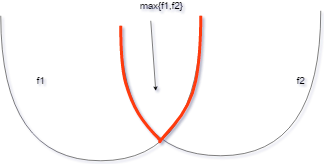
\includegraphics[]{1_3}
\item Composition with linear map.\\
$f \in cvx \R^n$, $A:\R^n \to \R^m$ is a linear map.
$f \circ A (x) = f(Ax) \in cvx \R^n$\\
\begin{align*}
f \circ A (x) & = f(A(\alpha x + (1-\alpha) y)) \\
& = f(A \alpha x + (1-\alpha) A y) \\
& \le \alpha f(Ax) + (a - \alpha) f(Ay)
\end{align*}
\end{itemize}

\section{Remarks}\index{Remarks}

This is an example of a remark.

\begin{remark}
The concepts presented here are now in conventional employment in mathematics. Vector spaces are taken over the field $\mathbb{K}=\mathbb{R}$, however, established properties are easily extended to $\mathbb{K}=\mathbb{C}$.
\end{remark}

%------------------------------------------------

\section{Corollaries}\index{Corollaries}

This is an example of a corollary.

\begin{corollary}[Corollary name]
The concepts presented here are now in conventional employment in mathematics. Vector spaces are taken over the field $\mathbb{K}=\mathbb{R}$, however, established properties are easily extended to $\mathbb{K}=\mathbb{C}$.
\end{corollary}

%------------------------------------------------

\section{Propositions}\index{Propositions}

This is an example of propositions.

\subsection{Several equations}\index{Propositions!Several Equations}

\begin{proposition}[Proposition name]
It has the properties:
\begin{align}
& \big| ||\mathbf{x}|| - ||\mathbf{y}|| \big|\leq || \mathbf{x}- \mathbf{y}||\\
&  ||\sum_{i=1}^n\mathbf{x}_i||\leq \sum_{i=1}^n||\mathbf{x}_i||\quad\text{where $n$ is a finite integer}
\end{align}
\end{proposition}

\subsection{Single Line}\index{Propositions!Single Line}

\begin{proposition} 
Let $f,g\in L^2(G)$; if $\forall \varphi\in\mathcal{D}(G)$, $(f,\varphi)_0=(g,\varphi)_0$ then $f = g$. 
\end{proposition}

\subsection{Paragraph of Text}\index{Examples!Paragraph of Text}

\begin{example}[Example name]
\lipsum[2]
\end{example}

%------------------------------------------------

\section{Exercises}\index{Exercises}

This is an example of an exercise.

\begin{exercise}
This is a good place to ask a question to test learning progress or further cement ideas into students' minds.
\end{exercise}

%------------------------------------------------

\section{Problems}\index{Problems}

\begin{problem}
What is the average airspeed velocity of an unladen swallow?
\end{problem}

%------------------------------------------------

\section{Vocabulary}\index{Vocabulary}

Define a word to improve a students' vocabulary.

\begin{vocabulary}[Word]
Definition of word.
\end{vocabulary}

%-------------------------------------------------------------------------------------------------
%   CHAPTER 5
%-------------------------------------------------------------------------------------------------
\part{Calcul numérique et discret}\index{Calcul numérique et discret}
\chapter{Nombres à virgule flottante}\index{Nombres à virgule flottante}
Dans les chapitres suivants, les nombres à virgule flottante sont au cœur des
calculs ; il convient de les étudier car leur comportement suit des règles précises.
Comment représenter des nombres réels en machine ? Comme ces nombres ne
peuvent pas en général être codés avec une quantité finie d’information, ils ne
sont pas toujours représentables sur un ordinateur : il faut donc les approcher
avec une quantité de mémoire finie.
Un standard s’est dégagé autour d’une approximation des nombres réels avec
une quantité fixe d’information : la représentation à virgule flottante.
Dans ce chapitre, on trouve : une description sommaire des nombres à virgule
flottante et des différents types de ces nombres disponibles dans SymPy, et la 
démonstration de quelques-unes de leurs propriétés. Quelques exemples montreront
certaines des difficultés qu’on rencontre en calculant avec les nombres à virgule
flottante, quelques astuces pour arriver parfois à les contourner, en espérant 
développer chez le lecteur une prudence bien nécessaire ; en conclusion, nous essayons
de donner quelques propriétés que doivent posséder les méthodes numériques pour
pouvoir être utilisées avec ces nombres.
\chapter{Algèbre linéaire numérique}
Dans ce chapitre on traite les aspects numériques de l'algèbre linéaire, algèbre linéaire symbolique étant présentée au chapitre 9. L'algèbre linéaire numérique joue un rôle prépondérant dans ce qu'il est convenu d'appeler le calcul scientifique, appellation impropre pour désigner des problèmes dont l'étude mathématique relève de l'analyse numérique : résolution approchée de systèmes d'équations différentielles, résolution approchée d'équations aux dérivées partielles, optimisation, traitement du signal, etc. La résolution numérique de la plupart de ces problèmes, même linéaires, est fondée sur des algorithmes formés de boucles imbriquées ; au plus profond de ces boucles, il y a très souvent la résolution d'un système linéaire. On utilise souvent
la méthode de Newton pour résoudre des systèmes algébriques non linéaires : là encore il faut résoudre des systèmes linéaires. 
La performance et la robustesse des méthodes d'algèbre linéaire numérique sont donc cruciales.


Ce chapitre comporte deux sections: la première section (§13.2) traite, sans être exhaustive, des problèmes les 
plus classiques (résolution de systèmes, calcul de valeurs propres, moindres carrés) ; dans la deuxième section on 
montre comment résoudre certains problèmes si on fait l'hypothèse que les matrices sont creuses. Cette dernière partie se veut
autant une initiation à des méthodes qui font partie d'un domaine de recherche actif qu'un guide d'utilisation.

\section{Matrices pleines}
class sympy.matrices.dense.\textbf{MutableDenseMatrix}
\subsection{Résolution de systèmes linéaires}
 \begin{flushleft}
 \textbf{Méthode à éviter} Ce qu'il ne faut (presque) jamais faire, c'est utiliser les formules de Cramer. Un raisonnement par récurrence montre que le coût du calcul du déterminant d'une matrice $n \times n$ en utilisant les formules de Cramer est de
l'ordre n! multiplications (et autant d'additions). Pour résoudre un système de taille $n$, ce sont $n + 1$ déterminants qu'il faut calculer. Prenons $n = 7$ :
\end{flushleft}
\begin{python}
In [1]: from sympy import factorial
In [2]: n = 7
In [3]: (n+1)*factorial(n+1)
Out[3]: 40320
 \end{python}
 \begin{flushleft}
  \textbf{Méthodes pratiques.} La résolution de systèmes linéaires $Ax = b$ est le plus souvent basée sur une factorisation de la matrice $A$ en un produit de deux matrices $A = M_{1}M_{2}$ , $M_{1} et M_{2}$ définissant des systèmes linéaires faciles à résoudre. Pour résoudre $Ax = b$, on résout alors successivement $M_{1}y = b$, puis $M_{2}x = y$.
 
 Par exemple $M_{1}$ et $M_{2}$ peuvent être deux matrices triangulaires ; dans ce cas, une fois la factorisation effectuée, il faut résoudre deux systèmes linéaires à matrice triangulaire. Le coût de la factorisation est bien plus élevé que celui de la résolution des deux systèmes triangulaires (par exemple $O\left(n^{3}\right)$ pour la factorisation \textit{LU} contre $O\left(n^{2}\right)$ pour la résolution des systèmes triangulaires). Il convient donc, dans le cas de la résolution de plusieurs systèmes avec la même matrice, de ne calculer qu'une seule fois la décomposition. Bien entendu, on n'inverse jamais une matrice pour résoudre un système linéaire, l'inversion demandant la factorisation de la matrice, puis la résolution de n systèmes au lieu d'un seul.
 \end{flushleft}
\subsection{Résolution directe}
\subsection{La décomposition \textit{LU}}
\begin{exercise}
\end{exercise}
\begin{exercise}

\end{exercise}
\subsection{La décomposition de Cholesky}
\begin{definition}
Une matrice symétrique $A$ est dite définie positive si pour tout vecteur $x$ non nul, ${}^t \!xAx>0$
\end{definition}
\begin{example}
SymPy utilise une méthode pour déterminer oui ou non une matrice donnée est positive ou pas.
\end{example}
\begin{definition}
Il existe une matrice triangulaire inférieure $N$ telle que $A = N^{t}N$. Cette factorisation est appelée décomposition de Cholesky. 
\end{definition}
Dans SymPy, elle se calcule en appelant la méthode cholesky()
\begin{example}

\end{example}
\begin{exercise}
A
\end{exercise}
\begin{exercise}
A
\end{exercise}
\begin{exercise}
A
\end{exercise}
\subsection{Décomposition \textit{QR}}
Soit $A \in \mathbb{R}^{n \times m}$, avec $n\geq m$ il s'agit ici de trouver des matrices $Q$ et $R$ telles que $A=QR$ ou $Q \in \mathbb{R}^{n \times m}$ est orthogonale $\left( {}^t\!Q.Q = I\right)$ et $R \in \mathbb{R}^{n \times m}$ est triangulaire supérieure. Bien sur, une fois la décomposition calculé, on peut s'en servir pour résoudre des systèmes linéaires si la matrice $A$ est carrée et inversible. 
\begin{exercise}
A
\end{exercise}
\begin{exercise}
A
\end{exercise}
\subsection{Valeurs propres, vecteurs propres}
Jusqu'à présent, nous n'avons utilisé que des méthodes directes (décomposition LU , QR, de Cholesky), qui fournissent une solution en un nombre fini d'opérations (les quatre opérations élémentaires, plus la racine carrée pour la décomposition de
Cholesky). Ce ne peut pas être le cas pour le calcul des valeurs propres : en effet, on peut associer à tout polynôme une matrice dont les valeurs propres sont les racines du polynôme ; mais on sait qu'il n'existe pas de formule explicite pour le calcul des racines d'un polynôme de degré supérieur ou égal à $5$, formule que donnerait précisément une méthode directe. D'autre part, former le polynôme caractéristique pour en calculer les racines serait extrêmement coûteux; notons toutefois que l'algorithme de Faddeev-Le Verrier permet de calculer le polynôme caractéristique d'une matrice de taille $n$ en $O\left(n^{4}\right)$ opérations, ce qui est malgré tout considéré comme bien trop coûteux. Les méthodes numériques
utilisées pour le calcul de valeurs et de vecteurs propres sont toutes itératives. On va donc construire des suites convergeant vers les valeurs propres (et les vecteurs propres) et arrêter les itérations quand on sera assez proche de la
solution
\begin{exercise}
A
\end{exercise}
\begin{exercise}
A
\end{exercise}
\begin{exercise}
A
\end{exercise}
\section{Matrices creuses}
Les matrices creuses sont très fréquentes en calcul scientifique : le caractère creux (sparsity en anglais) est une propriété recherchée qui permet de résoudre des problèmes de grande taille, inaccessibles avec des matrices pleines

\subsection{Origine des systèmes creux}
\begin{flushright}
\textbf{Problèmes aux limites.} L'origine la plus fréquente est la discrétisation d'équations aux dérivées partielles. Considérons par exemple l'équation de Poisson (équation de la chaleur stationnaire) :
\end{flushright}
\[
-\Delta u = f
\]
où $u= u\left(x, y\right)$, $f=f\left(x, y\right)$,
\[
\Delta u := \frac{\partial^{2}u}{\partial x^{2}} + \frac{\partial^{2}u}{\partial y^{2}}
\]
L'équation est posée dans le carré $\left[0, 1\right]^{2}$, et munie de conditions aux limites $u=0$ sur le bord du carré. L'analogue en dimension un est le problème
\begin{equation}
-\frac{\partial^{2}u}{\partial x^{2}} = f,
\end{equation}
avec $u\left(0\right) = u\left(1\right) = 0$.

Une des méthodes les plus simples pour approcher la solution de cette équation consiste à utiliser la méthode des différences finies : on découpe l'intervalle $\left[0, 1\right]$ en un nombre fini $N$ d'intervalles de pas h constant. On note $u_{i}$ la valeur approchée de u au point $x_{i} = ih$. On approche la dérivée de $u$ par $\left(u_{i+1} - u_{i}\right) \diagup h$ et sa dérivée seconde par
\[
\frac{\left(u_{i+1}-u_{i}\right)/h - \left(u_{i}-u_{i+1}\right)/h} {h} = \frac{u_{i+1}-2u_{i}+u_{i-1}}{h^{2}}
\]
On voit immédiatement que les $u_{0},..., u_{N}$ , qui approchent $u$ aux points $ih$, satisfont un système linéaire n'ayant que $3$ termes non nuls par ligne (et dont on peut vérifier que la matrice est symétrique définie positive).
\subsection{Valeurs propres, vecteurs propres}
\begin{flushright}
\textbf{La méthode de la puissance itérée.} La méthode de la puissance itérée est particulièrement adaptée au cas de très grandes matrices creuses ; en effet il suffit de savoir effectuer des produits matrice-vecteur (et des produits scalaires) pour savoir implanter l'algorithme. À titre d'exemple, revenons aux marches aléatoires sur un graphe creux, et calculons la distribution stationnaire, par la méthode de la puissance itérée
\end{flushright}

\chapter{Intégration numérique}\index{Intégration numérique}
Ce chapitre traite le calcul numérique d’intégrales (§14.1) ainsi que la résolution
numérique d'équations différentielles ordinaires (§14.2) avec SymPy. Nous rappelons
des bases théoriques des méthodes d’intégration, puis nous détaillons les fonctions
disponibles et leur usage (§14.1.1). Le calcul symbolique d’intégrales avec SymPy a été traité précédemment (§2.3.8), et ne sera que mentionné rapidement ici comme une possibilité de calculer la
valeur numérique d’une intégrale. Cette approche « symbolique puis numérique »,
lorsqu’elle est possible, constitue une des forces de SymPy et est à privilégier car le
nombre de calculs effectués, et donc d’erreurs d’arrondi, est en général moindre
que pour les méthodes d’intégration numérique. Nous donnons une rapide introduction aux méthodes classiques de résolution d’équations différentielles, puis le traitement d’un exemple (§14.2.1) débutera l’inventaire des fonctions disponibles en SymPy (§14.2.2).

On s’intéresse au calcul numérique d’intégrales de fonctions réelles ; pour une
fonction $f : I \longrightarrow R$, où $I$ est un intervalle de $\mathbb{R}$, on veut calculer :
\[
\int_{I} f\left(x\right).
\]

Par exemple, calculons
\[
 \int_{1}^{3} x^{2}e^{-x^{2}}\cos\left(x\right) dx.
\] 

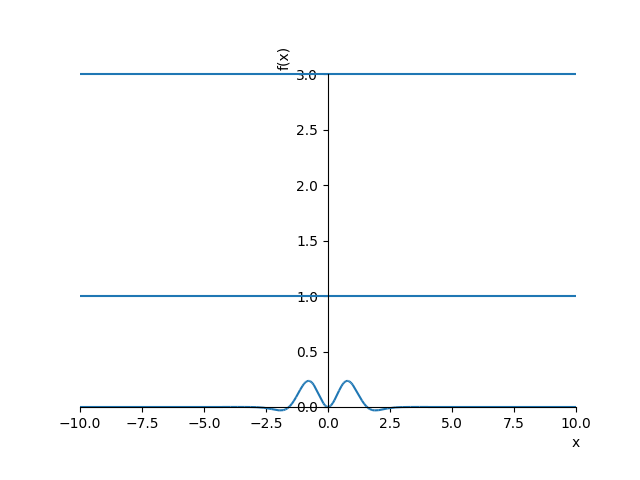
\includegraphics[scale=0.6]{../Pictures/Figure_1.png} 
\begin{python}
from sympy.abc import x
from sympy import integrate
from sympy.plotting import plot
f = x**2*exp(-x**2)*cos(x)
N(integrate(f, (x, 1, 3))
0.0306905101632536
plot(f, (1, 3, fill='axis'))
\end{python}

La fonction integrate calcule l’intégrale symbolique de l’expression, il faut
demander explicitement une valeur numérique pour l’obtenir.
\\
Il est aussi, en principe, possible de calculer des intégrales sur un intervalle
dont les bornes sont infinies :
\begin{python}
from sympy.abc import x
from sympy import sin, oo
N(integrate(sin(x**2)/(x**2), (x, 1, oo))
0.285736646322853
plot(sin(x**2)/(x**2), x, 1, 10, fill='axis')
\end{python}

\subsection{Equation and Text}\index{Examples!Equation and Text}

\begin{example}
Let $G=\{x\in\mathbb{R}^2:|x|<3\}$ and denoted by: $x^0=(1,1)$; consider the function:
\begin{equation}
f(x)=\left\{\begin{aligned} & \mathrm{e}^{|x|} & & \text{si $|x-x^0|\leq 1/2$}\\
& 0 & & \text{si $|x-x^0|> 1/2$}\end{aligned}\right.
\end{equation}
The function $f$ has bounded support, we can take $A=\{x\in\mathbb{R}^2:|x-x^0|\leq 1/2+\epsilon\}$ for all $\epsilon\in\intoo{0}{5/2-\sqrt{2}}$.
\end{example}


\chapter{Delta Dirac}
\chapter{Série de Fourier}

\chapter{Transformation d'intégrale}
 \section{Transformation de Fourier}
 Nous pouvons calculer des transformations de Fourier en utilisant la fonction SymPy fourier\_transform:

 \begin{exercise}
 \end{exercise}
 \begin{exercise}
 \end{exercise}
 \begin{exercise}
 \end{exercise}
  \subsection{Transformation de Fourier inverse}
  \begin{exercise}
 \end{exercise}
 \begin{exercise}
 \end{exercise}
 \section{Transformation de Laplace}
 \begin{python}
 \end{python}
 \begin{exercise}
 \end{exercise}
 \section{Transformation de Mellin}
 \begin{example}
  La transformée d'une distribution de Dirac ${\displaystyle \delta (x-a)}$, avec $a > 0$, est une fonction exponentielle ${\displaystyle s\mapsto a^{s-1}}$.
 \end{example}
 \begin{python}
 \end{python}
 \begin{example}
  La transformée de Mellin de la fonction ${\displaystyle f\,:\,x\mapsto \mathrm {H} (a-x)} {\displaystyle f\,:\,x\mapsto \mathrm {H} (a-x)}$, avec $a > 0$, est la fonction ${\displaystyle s\mapsto {\frac {a^{s}}{s}}} {\displaystyle s\mapsto {\frac {a^{s}}{s}}}$ sur le demi-plan $Re (s) > 0$
(où $H$ est la fonction de Heaviside, $f(x) = 1$ si $0 < x < a et f (x) = 0 si x > a$).
 \end{example}
 \begin{python}
 \end{python}
 \begin{example}
%   La transformée de Mellin de la fonction ${\frac {1}{\mathrm {e} ^{x}-1}}}$ est la fonction ${\displaystyle s\mapsto \Gamma (s)\zeta (s)}$ sur le demi-plan $Re (s) > 1$
 \end{example}
 \begin{python}
 \end{python}
 \subsection{Transformation de melin inverse}
 \section{Transfomation de Henkel}
 La transformée de Hankel (d'ordre zéro) est une transformée intégrale équivalente à une transformée de Fourier à deux dimensions avec un noyau intégral à symétrie radiale, appelée également transformation de Fourier-Bessel. Il est défini comme
 \[
 g \left(u, v \right)	= F_{r}\left[\left(r\right)\right]\left(u, v\right)
 \]
 \subsection{Transformation de Henkel inverse}
 
\chapter{Équations non linéaires}\index{Équations non linéaires}
Ce chapitre explique comment résoudre une équation non linéaire avec SymPy.
Dans un premier temps on étudie les équations polynomiales et on montre les
limitations de la recherche de solutions exactes. Ensuite on décrit le fonctionnement
de quelques méthodes classiques de résolution numérique. Au passage on indique
quels sont les algorithmes de résolution numérique implémentés dans SymPy.
Qu'est ce que non-linéaire et qu'est ce que une \'equation alg\'ebrique

Une \'equation alg\'ebrique est un polyn\^ome de la forme $P(x)$

\begin{equation}
\exp(-x)\sin(x) = \cos(x)
\end{equation}
\section{Équations algébriques}
%-------------------------------------------------

\section{Figure}\index{Figure}

\begin{table}[h]
\centering
\begin{tabular}{l l l}
\toprule
\textbf{Treatments} & \textbf{Response 1} & \textbf{Response 2}\\
\midrule
Treatment 1 & 0.0003262 & 0.562 \\
Treatment 2 & 0.0015681 & 0.910 \\
Treatment 3 & 0.0009271 & 0.296 \\
\bottomrule
\end{tabular}
\caption{Table caption}
\end{table}

%
%\begin{figure}[h]
%\centering\includegraphics[scale=0.5]
%\caption{Figure caption}
%\end{figure}

%----------------------------------------------------------------------------------------
\part{Combinatoire}

Les sujets de ce chapitre sont du néanmoins axées sur des questions ou l'approche mathématique et 
physique et demandé 

\chapter{Permutations}\index{Permutations}
Une permutation, également appelée "numéro d'agencement" ou "ordre", est un agencement des éléments d'une liste ordonnée dans un mappage un-à-un avec lui-même. La permutation d'un arrangement donné est donnée en indiquant les positions des éléments après le réarrangement. Par exemple, si on commençait par les éléments $\left[x, y, a, b\right]$ (dans cet ordre) et qu'ils étaient réordonnés sous la forme $\left[x, y, b, a\right]$, la permutation serait alors $\left[0, 1, 3, 2\right]$ . Notez que (dans SymPy) le premier élément est toujours désigné par $0$ et que la permutation utilise les indices des éléments dans l'ordre d'origine, et non les éléments ($a$, $b$, etc.) eux-mêmes.
\chapter{Groupe symmetrique}

 \begin{python}
  from sympy.combinatorics.named_groups import SymmetricGroup
  G = SymmetricGroup(4)
  G.is_group
  G.order()
  list(G.generate_schreier_sims(af=True))
 \end{python}
\chapter{Groupe Abélien}

%----------------------------------------------------------------------------------------
\part{Physique}
\chapter{Chaos}\index{Mouvement d'un pendule}
Prenons une pause dans l'apprentissage de nouvelles techniques et algorithmes informatiques
pour un peu, et passer du temps en utilisant ce que nous avons appris jusqu'à présent pour enquêter sur quelque chose d'intéressant. Nous allons commencer avec quelque chose de familier le pendule double.
\section{Mouvement d'un double pendule}
\section{Cinétique des gaz}


\chapter{M\'ecanique et information quantique}
\href{https://arxiv.org/pdf/1812.09167.pdf}{Quantum}

 

%----------------------------------------------------------------------------------------
%	Technique Avancée
%----------------------------------------------------------------------------------------

\part{Annexe}
\chapter{Programmation Orientée Objet}\index{Programmation Orientée Objet}
\chapter{D\'ecorateurs}
Les d\'ecorateurs un m\'ecanisme incontournable pour \'ecrire de tr\'es bon code et purement 
lisible et portable
\chapter{Optimisation du code}
Sans aucun doute l'usage de la programmation symbolique avec ce que en a vue plus haut, ralentisse
grandement l'exécution du programme, donc en gagne sur le coté sûreté, élégance
et maintenance du code et d'autre part en perd complètement la vitesse; penser à des centaine de ligne
de code si vous voulez programmé un robot, voiture ou des objets connectés qui implémente des
algorithmes mathématiques et qui de demande beaucoup de ressource est un temps de retour très élevées
\subsection{Cython}
Cython (http://www.cython.org/ ) est un métalangage qui permet de combiner du code
Python et des types de donn\'ees C, pour concevoir des extensions compilables pour
Python.
Dans un module Cython, il est possible de définir des variables C directement dans
le code Python et de définir des fonctions C qui prennent en paramètre des
variables C ou des objets Python.
Cython contr\^ole ensuite de manière transparente la génération de l’extension C, en
transformant le module en code C par le biais des API C de Python.
Toutes les fonctions Python du module sont alors automatiquement publiées.
Le gain de temps dans la conception introduit par Cython est considérable : toute la
mécanique habituellement mise en œuvre pour créer un module d’extension est
entièrement gérée par Cython.
Ainsi, la fonction max() du module calculs.c pr\'ec\'edemment présent\'ee devient :

Les fichiers Cython ont par convention l’extension pyx, en référence à l’ancien nom.

setup.py pour calculs.pyx

\begin{python}
from distutils.core import setup
from distutils.extension import Extension
from Cython.Distutils import build_ext

extension = Extension("calculs", ["calculs.pyx"])

setup(name="calculs", ext_modules=[extension],cmdclass={'build_ext': build_ext})

\end{python}

\subsection{Theano}
Theano est une biblioth\'eque pour l'acc\e'ration du code lent en Python, tr\'es importante et intéressante
elle offre une syntaxe très particulière.
\subsection{PyQt}

%----------------------------------------------------------------------------------------
%	BIBLIOGRAPHY
%----------------------------------------------------------------------------------------
\chapter*{Bibliography}
\addcontentsline{toc}{chapter}{\textcolor{ocre}{Bibliography}} % Add a Bibliography heading to the table of contents

%------------------------------------------------

\section*{Articles}
\addcontentsline{toc}{section}{Articles}
\printbibliography[heading=bibempty,type=article]

%------------------------------------------------

\section*{Books}
\addcontentsline{toc}{section}{Books}
\printbibliography[heading=bibempty,type=book]

%----------------------------------------------------------------------------------------
%	INDEX
%----------------------------------------------------------------------------------------

\cleardoublepage % Make sure the index starts on an odd (right side) page
\phantomsection
\setlength{\columnsep}{0.75cm} % Space between the 2 columns of the index
\addcontentsline{toc}{chapter}{\textcolor{ocre}{Index}} % Add an Index heading to the table of contents


\section{Index}

\end{document}
